% Template: IEEEtran, journal mode (IEEE Internet of Things Journal)
\documentclass[journal]{IEEEtran}

\usepackage{amsmath,amssymb,amsfonts}
\usepackage{graphicx}
\usepackage{booktabs}
\usepackage{array}
\usepackage{cite}
\usepackage{url}
\usepackage{xurl}
\usepackage{tikz}
\usetikzlibrary{arrows.meta,positioning,fit,calc,shapes.geometric,backgrounds}
% Colour-blind-safe palette (Okabe--Ito)
\definecolor{cReq}{RGB}{0,114,178}    % blue: request path
\definecolor{cPred}{RGB}{0,158,115}   % green: prediction stages
\definecolor{cCache}{RGB}{230,159,0}  % orange: cache storage
\definecolor{cPlat}{RGB}{204,121,167} % purple: platform profile
\definecolor{cUser}{RGB}{86,180,233}  % sky blue: users
\definecolor{cCP}{RGB}{120,120,120}   % grey: content provider
\definecolor{cHist}{RGB}{213,94,0}    % vermillion: request history

\newtheorem{assumption}{Assumption}
\newtheorem{definition}{Definition}
\newtheorem{proposition}{Proposition}
\newtheorem{remark}{Remark}

\newcommand{\U}{\mathcal{U}}
\newcommand{\F}{\mathcal{F}}
\newcommand{\X}{\mathcal{X}}
\newcommand{\Pset}{\mathcal{P}}
\newcommand{\J}{\mathcal{J}}
\newcommand{\M}{\mathcal{M}}
\newcommand{\R}{\mathcal{R}}
\newcommand{\Hist}{\mathcal{H}}
\newcommand{\Kset}{\mathcal{K}}
\newcommand{\bpi}{\boldsymbol{\pi}}
\newcommand{\ind}{\mathbf{1}}
\newcommand{\rmsub}[1]{\mathrm{#1}}
\newcommand{\tbd}[1]{\textcolor{red}{[TBD\if\relax\detokenize{#1}\relax\else: #1\fi]}}

\begin{document}

\title{TinyML for Edge Caching: How the Hardware Platform Shapes the Gain}

\author{Sameh~Hosny%
\thanks{S. Hosny is with the Electrical and Computer Engineering Department, American University of Armenia, Yerevan, Armenia (e-mail: sameh.hosny@aua.am; ORCID: 0000-0002-1672-7250).}}

\markboth{IEEE Internet of Things Journal}%
{Hosny: tinyML for Edge Caching: How the Hardware Platform Shapes the Gain}

\maketitle

\begin{abstract}
Learned caching models are usually evaluated on server hardware, yet many edge caches run on microcontrollers, where a model takes time to decide, shares a few kilobytes of memory with the request history, and consumes energy that may exceed the backhaul energy it saves. We model the caching decisions of an edge node as a pipeline of four stages (popularity prediction, admission and eviction, next-request prediction, and next-cell prediction), and each platform by a profile of its speed, memory, and energy, with a queueing model of decision time. We define a benchmark that selects the best model and platform for each stage and builds an energy-neutral and a hit-ratio-oriented pipeline, and we derive when a tinyML stage reduces the system energy. On four classes of microcontrollers and on a synthetic and a real movie-rating trace, only admission and eviction pays off on its own: it raises the hit ratio over ARC by 1.8 to 1.9 points on the synthetic trace and by 1.1 to 1.3 points on the real trace while saving energy. Behind it, next-request prefetching doubles the gain on the synthetic trace to 3.7 points at the cost of up to 32\% more backhaul traffic, but it does not help on the real trace. The platform hardly changes the hit-ratio gain but sets its energy cost: a platform with a neural accelerator is the best choice for every stage that benefits, and admission and eviction saves energy above 4~nJ per backhaul byte on it, against 0.7~$\mu$J on a Cortex-M4.
\end{abstract}

\begin{IEEEkeywords}
Edge caching, tinyML, microcontrollers, embedded machine learning, content popularity prediction, energy efficiency, Internet of Things.
\end{IEEEkeywords}

\IEEEpeerreviewmaketitle

\section{Introduction}\label{sec:intro}

\IEEEPARstart{T}{iny} machine learning (tinyML) is the execution of machine learning models on microcontroller-class devices, which have kilobytes of on-chip memory and operate within the power budget of battery-powered or energy-harvesting equipment \cite{sanchez2020,david2021,banbury2021}. A tinyML model is trained offline on a server, compressed, typically by 8-bit integer quantization \cite{jacob2018}, and deployed to the device, where it performs inference locally. Optimized kernels for Cortex-M processors \cite{lai2018}, interpreter-based inference frameworks \cite{david2021}, joint design of network architectures and inference engines \cite{lin2020}, kilobyte-sized recurrent models \cite{kusupati2018}, and low-power processors with parallel cores and neural accelerators \cite{flamand2018} have made such deployments practical.

Edge caching stores popular content at nodes close to the users, such as small base stations, gateways, and user devices, so that repeated requests are served without crossing the backhaul \cite{golrezaei2013,bastug2014,shi2016}. Its gain depends on how well the cache anticipates the demand. Proactive schemes therefore estimate content popularity and user behavior, including mobility, to decide what to store and when \cite{bastug2014,hosny2016allerton,hosny2016globecom}. Increasingly, these estimates are produced by learned models, such as deep networks for popularity prediction \cite{thar2018,kianfar2025} and learned eviction policies \cite{song2020}; surveys of this line of work are given in \cite{chang2018,shuja2021}.

Learned caching methods are usually designed and evaluated under the assumption that the model runs on server-class hardware. In DeepMEC, for example, the models are trained and executed in a cloud data center, and the resulting caching decisions are sent to the base stations \cite{thar2018}. LRB is implemented in a production cache server, and its overhead is measured on CDN servers \cite{song2020}. Many edge caches, however, are hosted on low-power nodes, such as IoT gateways, roadside units, or battery-powered devices, whose processors may be microcontrollers. When the caching model runs on such a node, it incurs costs that server-based evaluations do not capture. A decision takes time to compute, and requests that arrive in the meantime are served according to an outdated decision. The model occupies memory that the firmware and the cache index also need. Finally, every decision consumes energy, which may offset the backhaul energy that a better caching decision saves.

TinyML makes it possible to place caching models on such nodes, yet the existing literature does not show how much of the caching gain survives these costs. The standard tinyML benchmark evaluates isolated inference tasks, namely keyword spotting, visual wake words, image classification, and anomaly detection, in terms of accuracy, latency, and energy \cite{banbury2021}. It does not measure the effect of an on-device model on the performance of a networked system. Studies on learning-based caching, in turn, report hit ratios and backhaul savings but do not model the platform on which the model is executed. A system designer therefore cannot tell which caching decisions benefit from tinyML, which hardware platform is adequate for each decision, and under which conditions on-device inference costs more energy than it saves. To the best of our knowledge, these questions have not been answered in a systematic and reproducible way.

In this paper, we address this gap with a benchmark and analysis study of tinyML in edge caching. We model the caching decisions of an edge cache node as a pipeline of four stages: popularity prediction, admission and eviction, next-request prediction, and next-cell prediction. Each stage can be implemented by a conventional non-learned method or by a tinyML model. The hardware platform of the node is described by a set of parameters, its \emph{platform profile}, which captures the speed, memory, and energy consumption of the platform. The platform profiles are obtained from datasheets, published measurements, compiler estimates, and instruction-level cycle models, so that every hardware result can be reproduced without access to the boards. We evaluate the benchmark on a synthetic trace with controlled popularity drift, user mobility, and request successions, and on a trace built from the MovieTweetings dataset of movie ratings posted on Twitter \cite{dooms2013}. We first measure the gain of each stage over its non-learned baseline on each platform, then select the best model and platform for each stage, and finally evaluate the combined pipeline end to end.

The study answers the three questions raised above. Only admission and eviction benefits from tinyML on its own; next-request prefetching benefits only behind a learned admission stage and only where the demand has regular successions, and popularity and next-cell prediction do not benefit. A platform with a neural accelerator, here a Cortex-M55 with an Ethos-U55, is the most adequate for every stage that benefits: it matches the hit ratio of the other platforms at the lowest node energy, whereas the smallest platform can host only the smaller admission model. On-device inference costs more energy than it saves when the backhaul is cheaper than the break-even energy per byte of Proposition~\ref{prop:breakeven}, which ranges from 4~nJ on the accelerated platform to 0.7~$\mu$J on the Cortex-M4, and it always does so for prefetching, which buys hit ratio and delay with backhaul bytes.

The main contributions of this paper are as follows.
\begin{itemize}
\item We formulate a platform-aware model of an edge cache whose decisions are made by a pipeline of learned stages. The model represents the time that each decision takes through an explicit queueing and staleness model, so that the speed of the platform affects the hit ratio. It also accounts for the memory that the models and the request history share on the node and for the energy that each model consumes (Section~\ref{sec:system}).
\item We define a benchmark protocol that isolates the contribution of each stage, selects the best model and platform for each stage, and builds two pipelines: an energy-neutral one, which may not use more energy than the baseline, and a hit-ratio-oriented one, which evaluates the prefetching stages behind the learned admission stage and reports the energy it costs.
\item We derive a necessary and sufficient condition under which a tinyML stage reduces the energy of the system, together with the minimum request rate at which it does so (Proposition~\ref{prop:breakeven}).
\item We evaluate the benchmark across four classes of microcontroller platforms, from Cortex-M cores without accelerators to devices with neural accelerators and parallel RISC-V clusters, on a synthetic trace and on a trace of real movie ratings, and we answer the research questions with the best model and platform for each stage and a design procedure (Sections~\ref{sec:results} to~\ref{sec:guidelines}).
\item We release the simulator, the platform profiles, the trained models, the traces, and the experiment configurations at \url{https://github.com/sshawky78AUA/tinyML-Edge-Caching}, so that all results can be reproduced.
\end{itemize}

The rest of the paper is organized as follows. Section~\ref{sec:related} reviews related work. Section~\ref{sec:system} presents the system model, and Section~\ref{sec:problem} formulates the problem and derives the energy break-even condition. Section~\ref{sec:platforms} describes the hardware platforms and how their profiles are obtained, and Section~\ref{sec:setup} describes the simulation setup. Sections~\ref{sec:results} and~\ref{sec:hw} present the results and the hardware analysis. Section~\ref{sec:guidelines} answers the research questions and derives design guidelines, Section~\ref{sec:threats} discusses threats to validity, and Section~\ref{sec:conclusion} concludes the paper.

\section{Related Work}\label{sec:related}

\subsection{Edge Caching}
Caching content at the network edge was proposed to relieve the backhaul and to reduce the delay of content delivery. Golrezaei \emph{et al.} \cite{golrezaei2013} introduced femtocaching, in which helper nodes with large storage and limited backhaul cache popular videos, and showed that user devices can also act as caches through device-to-device (D2D) communication. Maddah-Ali and Niesen \cite{maddahali2014} characterized the fundamental limits of caching and showed that coded delivery adds a global caching gain to the local gain of conventional schemes. Ba\c{s}tu\u{g} \emph{et al.} \cite{bastug2014} advocated proactive caching, in which base stations and user devices store content in advance according to predicted popularity. User mobility has also been incorporated into the caching decision, for example by letting the service provider exploit the demand and mobility statistics of the users when it designs D2D caching policies \cite{hosny2016allerton,hosny2016globecom}. These works establish the gains of edge caching under analytical models of demand and mobility, but they do not model the computational cost of making the caching decisions.

\subsection{Learning-Based Caching}
Chang \emph{et al.} \cite{chang2018} discussed how large amounts of data can be used at the network edge for popularity estimation and proactive caching, and Shuja \emph{et al.} \cite{shuja2021} surveyed machine learning for edge caching with a taxonomy based on the learning technique, the caching strategy, and the type of edge network. Deep models have been proposed for popularity prediction. DeepMEC \cite{thar2018} predicts future popularity with deep networks that are trained and executed in the cloud, and CacheMamba \cite{kianfar2025} uses a selective state-space model to rank the files most likely to be requested and compares its accuracy and computational cost with those of a Transformer. In content distribution networks, LRB \cite{song2020} uses machine learning to approximate Belady's offline replacement rule \cite{belady1966}; it was implemented in a production cache server and evaluated on production traces, including a Wikipedia trace that was released with the paper. Learned policies are commonly compared with adaptive heuristics such as ARC \cite{megiddo2003}, and public traces, such as those of 153 in-memory cache clusters at Twitter \cite{yang2020}, allow them to be evaluated on real workloads. In all of these works the model runs on a server or in the cloud, and none evaluates how the hardware of a low-power cache node limits its gain.

\subsection{TinyML Platforms and Benchmarks}
Sanchez-Iborra and Skarmeta \cite{sanchez2020} reviewed the tinyML ecosystem and the frameworks available for integrating machine learning into microcontroller-based objects. Several techniques make this integration feasible. CMSIS-NN \cite{lai2018} provides neural network kernels for Arm Cortex-M processors and reports, for a convolutional network, a 4.6-fold improvement in throughput and a 4.9-fold improvement in energy efficiency. TensorFlow Lite Micro \cite{david2021} is an interpreter-based inference framework that runs in a few kilobytes of memory across heterogeneous embedded platforms. MCUNet \cite{lin2020} designs the network architecture and the inference engine jointly to fit deep models into the memory of a microcontroller. Integer-only quantization \cite{jacob2018} reduces the memory footprint of a model by a factor of almost four and enables inference on integer-only hardware, and FastGRNN \cite{kusupati2018} shows that recurrent models of a few kilobytes can run on microcontrollers. Beyond single-core devices, GAP-8 \cite{flamand2018} combines a RISC-V microcontroller with an eight-core cluster and a convolution accelerator, and GVSoC \cite{bruschi2021} simulates processors of this family with performance errors typically below 10\%. The MLPerf Tiny benchmark \cite{banbury2021} measures the accuracy, latency, and energy of tinyML systems on isolated inference tasks. It does not capture how the latency, memory, and energy of a platform affect a system in which the model is one component, which is the question that arises when a tinyML model makes caching decisions.

\subsection{TinyML for Data Management in IoT Systems}
Karras \emph{et al.} \cite{karras2024} proposed a set of tinyML algorithms for managing data in large-scale IoT systems; one of them, CacheEdgeML, uses predictive analytics to decide which data to cache. Their work concerns the storage and processing of sensor data within IoT networks. The present paper studies content caching between users and a content provider, and it quantifies how the hardware platform of the cache node shapes the caching gain.

\section{System Model}\label{sec:system}

We consider an edge caching network with three types of entities: a set of mobile users, an edge cache node (EN) located close to the users, for example in a gateway or a roadside unit, and a remote content provider (CP) that holds the full content catalogue. Users send their content requests to the EN. If the requested item is stored in the cache of the EN, it is delivered directly over the short access link. Otherwise, the EN retrieves the item from the CP over the backhaul link, which adds delay and consumes energy. The performance of the network therefore depends on which items the EN keeps in its cache and on how quickly it adapts its cache content to the demand of the users.

The caching decisions of the EN are made by a pipeline of four stages, each implemented by a non-learned method or by a tinyML model. All stages run on the processor of the EN, a low-power platform such as a microcontroller, whose speed, memory, and energy determine how quickly each stage decides, at what cost, and hence how much of the gain of a tinyML model is preserved.

The network, the request traces, and the structure of the pipeline are the same in all experiments, and the hardware platform is described by its \emph{platform profile}. An experiment changes only the implementation of the stages and the platform profile, so that the effect of each can be measured separately. Fig.~\ref{fig:system} illustrates the system, and Table~\ref{tab:notation} summarizes the notation.

\begin{figure*}[t]
\centering
\resizebox{\textwidth}{!}{%
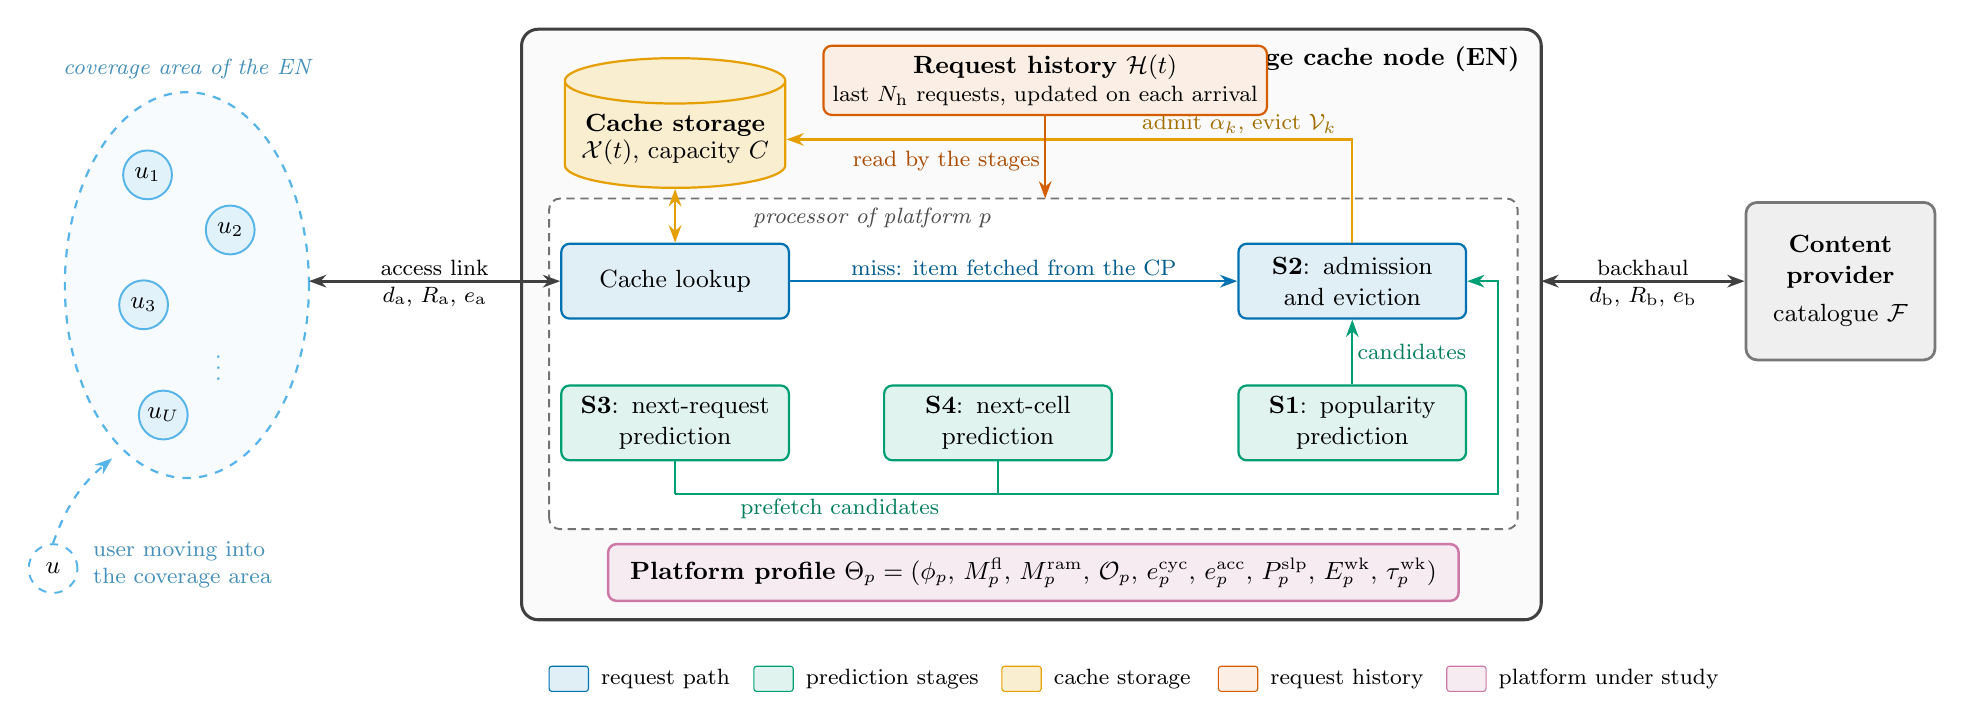
\begin{tikzpicture}[
  font=\small,
  >={Stealth[length=2.2mm,width=1.6mm]},
  stage/.style={draw, rounded corners=3pt, align=center, text width=2.75cm, minimum height=0.95cm, inner sep=2pt, line width=0.8pt},
  reqstage/.style={stage, draw=cReq, fill=cReq!12},
  predstage/.style={stage, draw=cPred, fill=cPred!12},
  user/.style={circle, draw=cUser, fill=cUser!18, minimum size=0.62cm, inner sep=0pt, line width=0.7pt},
  flow/.style={->, line width=0.8pt},
  dflow/.style={<->, line width=1.0pt},
  lab/.style={font=\footnotesize, align=center, inner sep=1.5pt},
  store/.style={cylinder, shape border rotate=90, aspect=0.22, draw=cCache, align=center, minimum width=2.8cm, minimum height=1.05cm, fill=cCache!18, line width=0.8pt}
]
% ---------------- users and coverage ----------------
\draw[dashed, draw=cUser, line width=0.8pt, fill=cUser!5] (0.5,0.35) ellipse (1.55cm and 2.45cm);
\node[lab, font=\footnotesize\itshape, text=cUser!80!black] at (0.5,3.1) {coverage area of the EN};
\node[user] (u1) at (0.00,1.75) {$u_1$};
\node[user] (u2) at (1.05,1.05) {$u_2$};
\node[user] (u3) at (-0.05,0.10) {$u_3$};
\node[text=cUser] at (0.90,-0.60) {$\vdots$};
\node[user] (uU) at (0.20,-1.30) {$u_U$};
\node[user, dashed, fill=white] (uo) at (-1.2,-3.25) {$u$};
\draw[flow, dashed, draw=cUser] (uo.north) to[bend left=15] (-0.45,-1.85);
\node[lab, anchor=west, align=left, text=cUser!80!black] at (-0.75,-3.2) {user moving into\\ the coverage area};

% ---------------- edge cache node ----------------
\draw[line width=1.1pt, rounded corners=6pt, draw=black!75, fill=black!2] (4.75,-3.9) rectangle (17.7,3.6);
\node[font=\small\bfseries, anchor=north east] at (17.55,3.5) {Edge cache node (EN)};
\node[store] (cache) at (6.7,2.2) {\textbf{Cache storage}\\[-1pt] $\X(t)$, capacity $C$};

\draw[densely dashed, rounded corners=4pt, line width=0.7pt, draw=black!55, fill=white] (5.1,-2.75) rectangle (17.4,1.45);
\node[lab, font=\footnotesize\itshape, text=black!70] at (9.2,1.2) {processor of platform $p$};

% request path
\node[reqstage] (look) at (6.7,0.4)  {Cache lookup};
\node[reqstage] (s2)   at (15.3,0.4) {\textbf{S2}: admission\\ and eviction};
% prediction stages
\node[predstage] (s3)   at (6.7,-1.4)  {\textbf{S3}: next-request\\ prediction};
\node[predstage] (s5)   at (10.8,-1.4) {\textbf{S4}: next-cell\\ prediction};
\node[predstage] (s1)   at (15.3,-1.4) {\textbf{S1}: popularity\\ prediction};

\draw[flow, draw=cReq] (look) -- node[lab, above, text=cReq!80!black] {miss: item fetched from the CP} (s2);
\draw[flow, draw=cPred] (s1) -- node[lab, right, text=cPred!80!black] {candidates} (s2);
\draw[dflow, draw=cCache] (look.north) -- (cache.south);
\draw[flow, draw=cCache] (s2.north) |- node[lab, above, pos=0.6, text=cCache!70!black] {admit $\alpha_k$, evict $\mathcal{V}_k$} (cache.east);
\node[draw=cHist, fill=cHist!10, rounded corners=3pt, align=center, minimum width=3.6cm, minimum height=0.8cm, line width=0.8pt] (hist) at (11.4,2.95) {\textbf{Request history} $\mathcal{H}(t)$\\[-1pt] {\footnotesize last $N_{\mathrm{h}}$ requests, updated on each arrival}};
\draw[flow, draw=cHist] (hist.south) -- node[lab, left, pos=0.55, text=cHist!80!black] {read by the stages} (11.4,1.45);
\draw[line width=0.8pt, draw=cPred] (s3.south) -- (6.7,-2.3);
\draw[line width=0.8pt, draw=cPred] (s5.south) -- (10.8,-2.3);
\draw[flow, draw=cPred] (6.7,-2.3) -- node[lab, below, pos=0.2, text=cPred!80!black] {prefetch candidates} (17.15,-2.3) |- (s2.east);

% platform profile
\node[draw=cPlat, fill=cPlat!15, rounded corners=3pt, minimum width=10.8cm, minimum height=0.72cm, align=center, line width=0.9pt] (prof) at (11.25,-3.3)
  {\textbf{Platform profile} $\Theta_p=(\phi_p,\, M^{\mathrm{fl}}_p,\, M^{\mathrm{ram}}_p,\, \mathcal{O}_p,\, e^{\mathrm{cyc}}_p,\, e^{\mathrm{acc}}_p,\, P^{\mathrm{slp}}_p,\, E^{\mathrm{wk}}_p,\, \tau^{\mathrm{wk}}_p)$};

% ---------------- content provider ----------------
\node[draw=cCP, fill=cCP!12, rounded corners=4pt, align=center, minimum width=2.4cm, minimum height=2.0cm, line width=1.0pt] (cp) at (21.5,0.4) {\textbf{Content}\\ \textbf{provider}\\[3pt] catalogue $\F$};

% ---------------- links ----------------
\draw[dflow, draw=black!75] (2.05,0.4) -- node[lab, above] {access link} node[lab, below] {$d_{\mathrm{a}},\,R_{\mathrm{a}},\,e_{\mathrm{a}}$} (look.west);
\draw[dflow, draw=black!75] (17.7,0.4) -- node[lab, above] {backhaul} node[lab, below] {$d_{\mathrm{b}},\,R_{\mathrm{b}},\,e_{\mathrm{b}}$} (cp.west);

% ---------------- legend ----------------
\begin{scope}[shift={(5.1,-4.65)}]
  \node[draw=cReq, fill=cReq!12, minimum width=0.5cm, minimum height=0.32cm, rounded corners=1pt] (l1) at (0.25,0) {};
  \node[lab, anchor=west] at (0.6,0) {request path};
  \node[draw=cPred, fill=cPred!12, minimum width=0.5cm, minimum height=0.32cm, rounded corners=1pt] at (2.85,0) {};
  \node[lab, anchor=west] at (3.2,0) {prediction stages};
  \node[draw=cCache, fill=cCache!18, minimum width=0.5cm, minimum height=0.32cm, rounded corners=1pt] at (6.0,0) {};
  \node[lab, anchor=west] at (6.35,0) {cache storage};
  \node[draw=cHist, fill=cHist!10, minimum width=0.5cm, minimum height=0.32cm, rounded corners=1pt] at (8.75,0) {};
  \node[lab, anchor=west] at (9.1,0) {request history};
  \node[draw=cPlat, fill=cPlat!15, minimum width=0.5cm, minimum height=0.32cm, rounded corners=1pt] at (11.65,0) {};
  \node[lab, anchor=west] at (12.0,0) {platform under study};
\end{scope}
\end{tikzpicture}}
\caption{System model. Users in the coverage area of the edge cache node (EN) send requests over the access link. The EN looks each request up in its cache storage. On a miss, it fetches the item from the content provider over the backhaul, while S2 decides whether to admit it. The four stages S1 to S4 run on the processor of the EN: S2 (blue) acts on each miss, and the prediction stages (green) run ahead of the requests and feed S2. The stages read the request history (vermillion), which holds the last $N_\mathrm{h}$ requests in the on-chip memory of the EN. The platform profile $\Theta_p$ (purple) describes the platform under study.}
\label{fig:system}
\end{figure*}

\subsection{Network and Content}\label{sec:network}

The system comprises a set of users $\U=\{1,\dots,U\}$, one edge cache node (EN), and a content provider (CP). The CP holds a catalogue $\F=\{1,\dots,F\}$, where item $f\in\F$ has size $s_f$ bytes. At time $t$ the EN stores a subset $\X(t)\subseteq\F$ of the catalogue, subject to the capacity constraint
\begin{equation}
\sum_{f\in\X(t)} s_f \le C, \qquad \forall t\ge 0,
\label{eq:capacity}
\end{equation}
where $C$ is the cache capacity in bytes.

Users communicate with the EN over an access link with propagation delay $d_\rmsub{a}$ and data rate $R_\rmsub{a}$, and the EN communicates with the CP over a backhaul link with propagation delay $d_\rmsub{b}$ and data rate $R_\rmsub{b}$. The time needed to transfer item $f$ depends on its size. It takes
\begin{equation}
d^\rmsub{a}_f = d_\rmsub{a} + \frac{s_f}{R_\rmsub{a}}
\label{eq:access_delay}
\end{equation}
to deliver item $f$ from the EN to a user, which we call the access delay of $f$, and
\begin{equation}
d^\rmsub{b}_f = d_\rmsub{b} + \frac{s_f}{R_\rmsub{b}}
\label{eq:backhaul_delay}
\end{equation}
to fetch item $f$ from the CP to the EN, which we call the fetch delay of $f$. Transferring item $f$ also consumes energy on each link. Delivering it over the access link consumes $E^\rmsub{a}_f=e_\rmsub{a}\,s_f$, and fetching it over the backhaul consumes $E^\rmsub{b}_f=e_\rmsub{b}\,s_f$, where $e_\rmsub{a}$ and $e_\rmsub{b}$ are the energies per transported byte of the access link and the backhaul, respectively.

Users are mobile and may enter or leave the coverage area of the EN. Mobility affects the system only through stage S4 of the pipeline, which predicts the users who are about to enter the coverage area, and it is described in Section~\ref{sec:pipeline}.

\begin{assumption}\label{as:storage}
Cached items reside in storage attached to the EN, such as external flash or a memory card, which is separate from the on-chip memory of its processor. The on-chip memory holds the firmware, the cache index, the request history, and the models of the pipeline.
\end{assumption}

Under Assumption~\ref{as:storage}, the models and the request history compete for processor memory with the firmware and the index, but they do not reduce the cache capacity $C$.

\begin{assumption}\label{as:links}
The access link and the backhaul are not congested: the delivery delay of a request does not depend on the other requests in progress.
\end{assumption}

Under Assumption~\ref{as:links}, each transfer obtains the full rate of its link, regardless of the load, and overlapping transfers proceed in parallel. We further assume that the EN forwards a fetched item to the user after receiving it completely. The resulting delivery delay of a request is given in \eqref{eq:request_delay}. Congestion would add a source of variation that is unrelated to the platform, which is the subject of this paper.

\subsection{Request Process}\label{sec:requests}

Rather than assuming a stochastic model of the requests, we drive the system with recorded request traces. A \emph{request} is a triple
\begin{equation}
r_k=(t_k,u_k,f_k)\in[0,\infty)\times\U\times\F,
\label{eq:request}
\end{equation}
which states that user $u_k$ requests item $f_k$ at time $t_k$. A \emph{trace} is a finite sequence of $K$ requests,
\begin{equation}
\R=(r_1,r_2,\dots,r_K), \qquad t_1\le t_2\le\dots\le t_K,
\label{eq:trace}
\end{equation}
indexed by $k\in\Kset=\{1,\dots,K\}$ in the order of arrival. Since a user may issue several requests, $u_k=u_{k'}$ may hold for $k\neq k'$, and likewise $f_k=f_{k'}$. Requests with equal time stamps keep the order in which they appear in the recorded trace, so the index $k$ fixes a unique processing order. If a trace does not identify individual users, all of its requests are attributed to a single aggregate user, i.e., $U=1$.

A user who waits too long for an item may request it again. We call such a repeated request a \emph{retry}. A retry does not represent new demand, so we do not treat it as a new request. Formally, when the trace identifies users, request $k$ is a retry if the same user requested the same item at most $\tau_\rmsub{r}$ earlier, that is, if there is a request $k'<k$ with $u_{k'}=u_k$, $f_{k'}=f_k$, and $t_k-t_{k'}\le\tau_\rmsub{r}$. Retries are removed from the trace before the simulation starts, so the set of removed requests depends only on the trace and not on the decisions of the EN. When the trace does not identify users, a retry cannot be distinguished from a request of another user for the same item, and no request is removed. In the rest of the paper, $\R$, $K$, and $\Kset$ refer to the trace after the retries are removed. Neither trace of Section~\ref{sec:setup} contains retries, so $\tau_\rmsub{r}$ does not affect the reported results.

At time $t$, the EN knows only the requests that have already arrived, and it stores only the most recent of them. Let $\Kset(t)=\{k\in\Kset: t_k<t\}$ be the indices of the requests that arrived before $t$. The \emph{request history} at time $t$ is the subsequence of the last $N_\rmsub{h}$ of these requests,
\begin{equation}
\Hist(t)=(r_k)_{k\in\Kset(t),\ k>|\Kset(t)|-N_\rmsub{h}},
\label{eq:history}
\end{equation}
which the EN keeps in a first-in, first-out buffer: when a request arrives, it enters the history, and the oldest request leaves once the history holds $N_\rmsub{h}$ requests. Each stored request occupies $b_\rmsub{r}$ bytes, so the history occupies $N_\rmsub{h}b_\rmsub{r}$ bytes of the on-chip memory of the EN. The length $N_\rmsub{h}$ is therefore limited by the memory of the platform, as specified in Section~\ref{sec:platform}. Since the history contains only requests with $t_k<t$, no stage uses information about future requests.

Each trace serves three purposes: to train the models, to select the best model for each stage, and to measure the final performance. To keep these purposes separate, the trace is divided in time into three consecutive parts. Given two instants $t_1<T_\rmsub{tr}<T_\rmsub{va}<t_K$, the index sets of the three parts are
\begin{equation}
\begin{aligned}
\Kset_\rmsub{tr}&=\{k\in\Kset:\ t_k< T_\rmsub{tr}\},\\
\Kset_\rmsub{va}&=\{k\in\Kset:\ T_\rmsub{tr}\le t_k< T_\rmsub{va}\},\\
\Kset_\rmsub{te}&=\{k\in\Kset:\ t_k\ge T_\rmsub{va}\},
\end{aligned}
\label{eq:split}
\end{equation}
and the corresponding subsequences of $\R$ are the \emph{training part} $\R_\rmsub{tr}=(r_k)_{k\in\Kset_\rmsub{tr}}$, the \emph{validation part} $\R_\rmsub{va}=(r_k)_{k\in\Kset_\rmsub{va}}$, and the \emph{test part} $\R_\rmsub{te}=(r_k)_{k\in\Kset_\rmsub{te}}$. The models are trained on $\R_\rmsub{tr}$, the best model for each stage is selected on $\R_\rmsub{va}$, and all reported results are computed on $\R_\rmsub{te}$. Training examples are generated by replaying $\R_\rmsub{tr}$ through the same request history that the EN keeps, so that each model is trained on the inputs that it receives after deployment. Each evaluation starts with a warm-up before its part begins (Section~\ref{sec:setup}), and the requests of the warm-up are not counted in any metric. The test part contains $K_\rmsub{te}=|\Kset_\rmsub{te}|$ requests and covers the time interval $[T_\rmsub{va},t_K]$ of duration $T_\rmsub{te}=t_K-T_\rmsub{va}$, so its mean request rate is $\lambda=K_\rmsub{te}/T_\rmsub{te}$. Since every request of $\R_\rmsub{tr}$ precedes every request of $\R_\rmsub{va}$, which in turn precedes every request of $\R_\rmsub{te}$, no model is trained or selected using requests that arrive after the requests on which it is evaluated. The synthetic trace of Section~\ref{sec:setup} follows the same definitions.

\begin{assumption}\label{as:openloop}
The requests do not depend on the decisions of the EN: the times, users, and items in the trace $\R$ are the same for every pipeline configuration and every platform.
\end{assumption}

Assumption~\ref{as:openloop} states that the EN observes the requests but does not influence them. Under this assumption, every pipeline configuration and every platform is evaluated on exactly the same sequence of requests, so a difference in performance between two evaluations can only come from the caching decisions and the platform. The assumption is also what allows us to drive the system with a recorded trace, since a recorded trace cannot react to the decisions of the cache under study. Trace-driven evaluations of caching policies rely on the same assumption \cite{megiddo2003,song2020}.

The assumption holds when the trace records demand that does not depend on the cache. This is the case for request traces recorded at a cache placed where the EN is, such as the Wikipedia CDN trace that the authors of LRB released with their paper \cite{song2020}, and it holds by construction for the synthetic trace of Section~\ref{sec:setup}. It also holds for the MovieTweetings trace of Section~\ref{sec:setup}, whose events are ratings that users post after watching a movie; whether a cache served the movie does not change when, or whether, a user rates it.

The assumption excludes one reaction of the users: a user whose request is served slowly may repeat it, and the EN under study may cause repetitions that the trace does not contain. Two properties of the model limit this effect. First, a repeated request is merged with the request that it repeats, so the item is fetched at most once and the repetition changes neither the cache nor the metrics. Second, the platform never delays a delivery: the cache lookup is served before any stage trigger, a hit is delivered without waiting for any stage, and a miss is fetched from the CP while S2 decides, in parallel, whether to admit the item. A platform can therefore change the number of repeated requests only through its hit ratio, as any caching policy does.

Let $\X_k$ denote the content of the cache immediately before request $k$ is processed. Request $k$ is a \emph{hit} if $f_k\in\X_k$, in which case $f_k$ is delivered from the cache. Otherwise, it is a \emph{miss}, and $f_k$ is fetched from the CP and delivered. We record the outcome by the indicator $h_k\in\{0,1\}$, which equals one if and only if request $k$ is a hit. The delay and the link energy of delivering the requested item to user $u_k$ are then
\begin{align}
d_k&=d^\rmsub{a}_{f_k}+\bigl(1-h_k\bigr)\,d^\rmsub{b}_{f_k}, \label{eq:request_delay}\\
E_k&=E^\rmsub{a}_{f_k}+\bigl(1-h_k\bigr)\,E^\rmsub{b}_{f_k}. \label{eq:request_energy}
\end{align}
For a hit, the item crosses only the access link. For a miss, it crosses the backhaul and then the access link, so both its delay and its energy add up over the two links. Only exact matches are served from the cache; delivering a semantically similar item in place of a missing one is left for future work.

\subsection{Time Model}\label{sec:time}

Time is continuous, and the state of the system changes only at discrete events. An event is the arrival of a request, the release of a stage trigger, the completion of a decision, or the completion of a backhaul fetch. The simulator processes the events in the order of their occurrence. Hence, every request is served at its own arrival time $t_k$, and every decision takes effect at the instant at which it is completed.

We do not divide time into slots, in which the requests of a slot are served together under one decision made at the start of the slot. A slotted model assumes that every decision is ready at the start of the slot in which it is used, so the decision latency $\tau_{m,p}$ of model $m$ on platform $p$, defined in \eqref{eq:latency}, has no effect as long as it is shorter than the slot, and two platforms whose latencies differ by orders of magnitude produce identical results. In the event-driven model, requests that arrive while a decision is computed are served according to the previous decision, so a slower platform serves more requests with outdated decisions, and the latency of each platform enters the results directly (Section~\ref{sec:timing}).

Stages S1 and S4, defined in Section~\ref{sec:pipeline}, are executed periodically, with periods $T_1$ and $T_4$. We refer to the interval between two consecutive executions of a periodic stage as an \emph{update epoch} of that stage. The output of a periodic stage remains fixed during an update epoch, whereas the other stages act on every request or miss as it occurs.

All performance metrics are averaged at two levels. First, each metric in Section~\ref{sec:metrics} is a time average over the test part $\R_\rmsub{te}$, that is, an average over all of its $K_\rmsub{te}$ requests or over its duration $T_\rmsub{te}$. Second, since the trace is fixed, the only source of randomness in an experiment is the training of the models. Each experiment is therefore repeated with independent training seeds, and we report the mean over the seeds together with its 95\% confidence interval. Because a time average conceals variations over time, such as those caused by popularity drift or by periods of high demand, we also report the hit ratio over consecutive windows of fixed length, as defined in \eqref{eq:window_hit}.

\subsection{Caching Pipeline}\label{sec:pipeline}

The caching decisions of the EN are made by a pipeline of four stages, indexed by $j\in\J=\{1,\dots,4\}$. At each of its trigger instants $t$, stage $j$ maps the history $\Hist(t)$, the cache state $\X(t)$, and the outputs of the other stages to an output $y_j(t)$. Table~\ref{tab:stages} defines the output, the trigger, and the non-learned baseline of each stage.

\begin{table*}[t]
\centering
\caption{Stages of the Caching Pipeline}
\label{tab:stages}
\small
\setlength{\tabcolsep}{4pt}
\begin{tabular}{@{}llll@{}}
\toprule
Stage & Output $y_j(t)$ & Trigger & Baseline $b_j$ \\
\midrule
S1: Popularity prediction & Request probability $\hat{p}_f(t)$ of each item within $W_1$ & Every $T_1$ & Exponentially weighted counts \\
S2: Admission and eviction & Admission $\alpha_k\in\{0,1\}$ and victim set $\mathcal{V}_k\subseteq\X(t)$ & Every miss and prefetch & Best of LRU, LFU, and ARC \\
S3: Next-request prediction & At most $L$ likely next items of user $u_k$ & Every request & No prefetching \\
S4: Next-cell prediction & Users entering the coverage area within $W_4$ & Every $T_4$ & No prediction \\
\bottomrule
\end{tabular}
\end{table*}

The stages interact through the data flow of Fig.~\ref{fig:system}. Stages S1, S3, and S4 generate prefetch candidates, namely the uncached items with the highest estimated popularity, the predicted next items of active users, and the predicted next items of users who are about to arrive. Stage S4 predicts which users will arrive, and S3 predicts what each of them will request first. When S3 uses its baseline, S4 prefetches instead the items that most often followed the user's latest item in the history. Every candidate passes through the admission rule of S2 before it is fetched and enters the cache, so the value of a prefetching stage depends on the admission policy. Since S1 prefetches with its baseline as well, the baseline configuration also prefetches. Prefetched items are transported over the backhaul, so their bytes and energy are charged to the system.

Stage S4 is the only stage that uses the location of the users. We denote by $\U(t)\subseteq\U$ the set of users in the coverage area of the EN at time $t$. Stage S4 therefore requires a trace that records where the users are. When a trace contains no user locations, as is the case for traces recorded at a single cache, S4 is disabled and its baseline is used.

Stage S3 predicts the next request of a user. Let $f$ be the latest item of user $u_k$. The candidates of S3 are the items that users requested right after $f$ in the history, and S3 estimates for each candidate the probability that it is the next item that $u_k$ requests. It prefetches the at most $L$ candidates whose probability is at least a threshold $\theta_3$. The other three stages predict whether an event occurs within a fixed time after the instant $t$ at which they act, called the \emph{prediction horizon} of the stage. Stage S1 estimates, for every item $f$, the probability $\hat p_f(t)$ that $f$ is requested at least once in the interval $(t,t+W_1]$. Stage S2 estimates, for the fetched item and for every cached item that it considers for eviction, the probability that the item is requested again in $(t,t+W_2]$; it admits the fetched item if this probability is at least a threshold $\theta_2$, and it evicts the cached items with the lowest probabilities. Stage S4 estimates, for every user $u\notin\U(t)$ in the cells adjacent to the coverage area, the probability that $u\in\U(t')$ for some $t'\in(t,t+W_4]$, and it predicts that $u$ will arrive if this probability is at least a threshold $\theta_4$. A horizon longer than the period of a periodic stage lets consecutive predictions overlap, so that a user who arrives just after the next execution of S4 has already been predicted, and it leaves time to fetch the prefetched items before they are requested. The values of the horizons and thresholds are given in Section~\ref{sec:setup}.

For each stage $j$, let $\M_j$ denote the set of candidate tinyML models and $b_j$ its baseline. A \emph{pipeline configuration} assigns one implementation to every stage,
\begin{equation}
\bpi=(m_1,\dots,m_4), \qquad m_j\in\M_j\cup\{b_j\}.
\label{eq:config}
\end{equation}
The baseline configuration is $\bpi^0=(b_1,\dots,b_4)$, and $\bpi^0[j\leftarrow m]$ denotes the configuration that coincides with $\bpi^0$ except that stage $j$ is implemented by model $m$.

\begin{assumption}\label{as:offline}
Every model is trained offline on $\R_\rmsub{tr}$, quantized to 8-bit integer arithmetic, and deployed to the EN, which performs inference only. The energy of receiving and storing a model update is modelled by $E^\rmsub{upd}_{m,p}$ in \eqref{eq:update}; the results reported here contain no updates.
\end{assumption}

Assumption~\ref{as:offline} reflects how tinyML models are developed and deployed in practice \cite{jacob2018,david2021}. Training needs floating-point arithmetic, stored activations, and repeated passes over the data, whereas inference needs one forward pass in integer arithmetic; a node with a few kilobytes of RAM, such as the Class~1 platform of Section~\ref{sec:platforms}, can do the second but not the first. The node therefore pays for inference and for receiving updates, and the cost of training is not counted. Quantization to 8-bit integers is the one number format that every platform in this study executes efficiently, since the Cortex-M3 has no floating-point unit \cite{st_f103} and the Ethos-U55 is built around 8-bit multiply-accumulate units \cite{arm_m55blog}. Every platform therefore runs the same quantized model and makes the same decisions, so differences in the results come from the latency, memory, and energy of the platform. Since the deployed models do not change during the test part, no model learns from the requests on which it is evaluated.

\subsection{Platform Model}\label{sec:platform}

Let $\Pset$ denote the set of hardware platforms under study. Platform $p\in\Pset$ is characterized by its profile
\begin{multline}
\Theta_p=\bigl(\phi_p,\, \phi^\rmsub{npu}_p,\, M^\rmsub{fl}_p,\, M^\rmsub{ram}_p,\, \mathcal{O}_p,\, e^\rmsub{cpu}_p,\, e^\rmsub{npu}_p,\\
e^\rmsub{acc}_p,\, P^\rmsub{slp}_p,\, \eta^\rmsub{ret}_p,\, E^\rmsub{wk}_p,\, \tau^\rmsub{wk}_p,\, e^\rmsub{rx}_p,\, e^\rmsub{fw}_p\bigr),
\label{eq:profile}
\end{multline}
where $\phi_p$ and $\phi^\rmsub{npu}_p$ are the clock frequencies of the processor and of its neural accelerator, $M^\rmsub{fl}_p$ and $M^\rmsub{ram}_p$ are the flash and RAM capacities, $\mathcal{O}_p$ is the set of operators supported by the platform toolchain, $e^\rmsub{cpu}_p$ is the energy of the platform per processor cycle, $e^\rmsub{npu}_p$ is the energy of the platform per accelerator cycle, including the processor while it waits for the accelerator, $e^\rmsub{acc}_p$ is the energy per off-chip memory access, $P^\rmsub{slp}_p$ is the sleep power, $\eta^\rmsub{ret}_p$ is the additional sleep power per byte of retained RAM on platforms that retain RAM selectively, and is zero on platforms whose sleep mode retains the whole RAM at the power $P^\rmsub{slp}_p$, $E^\rmsub{wk}_p$ and $\tau^\rmsub{wk}_p$ are the energy and the duration of a wake-up from sleep, and $e^\rmsub{rx}_p$ and $e^\rmsub{fw}_p$ are the energies per byte of receiving data over the radio and of writing it to flash. For a platform without an accelerator, the accelerator entries are not used. If the accelerator shares the clock of the processor, $\phi^\rmsub{npu}_p=\phi_p$.

Every entry of $\Theta_p$ is taken from the datasheet of the platform or from published measurements. All entries refer to one operating point per platform, namely the nominal supply voltage and clock frequency of its datasheet, which we report. This makes the profiles of different platforms directly comparable. Voltage and frequency scaling are outside the scope of this work.

Compiling model $m$ for platform $p$ yields its flash and RAM footprints, $\mu^\rmsub{fl}_{m,p}$ and $\mu^\rmsub{ram}_{m,p}$, and executing it in the simulator or emulator of $p$ yields, per inference, the number of processor cycles $N^\rmsub{cpu}_{m,p}$, the number of accelerator cycles $N^\rmsub{npu}_{m,p}$, and the number of off-chip memory accesses $A_{m,p}$. If the platform has no accelerator, or the model does not use it, $N^\rmsub{npu}_{m,p}=0$. Let $\Omega_m$ be the set of operators used by $m$, and let $M^\rmsub{fl}_0$ and $M^\rmsub{ram}_0$ be the memory reserved for the firmware and the cache index.

\begin{definition}\label{def:feasible}
Model $m$ is \emph{feasible} on platform $p$, written $\psi_{m,p}=1$, if $\Omega_m\subseteq\mathcal{O}_p$, $\mu^\rmsub{fl}_{m,p}\le M^\rmsub{fl}_p-M^\rmsub{fl}_0$, and $\mu^\rmsub{ram}_{m,p}\le M^\rmsub{ram}_p-M^\rmsub{ram}_0$. A configuration $\bpi$ with history length $N_\rmsub{h}$ is feasible on $p$ if every model in it satisfies the operator condition, $\sum_{j\in\J}\mu^\rmsub{fl}_{m_j,p}\le M^\rmsub{fl}_p-M^\rmsub{fl}_0$, and $N_\rmsub{h}b_\rmsub{r}+\sum_{j\in\J}\mu^\rmsub{ram}_{m_j,p}\le M^\rmsub{ram}_p-M^\rmsub{ram}_0$.
\end{definition}

The history and the models share the RAM of the platform. For a given configuration, we set $N_\rmsub{h}$ to the largest value that satisfies Definition~\ref{def:feasible}. A platform with more RAM can therefore keep a longer history, while a large model on a small platform leaves room only for a short one. Since $N_\rmsub{h}$ requests may cover a few seconds of a busy trace or several hours of a quiet one, we also report the time span $N_\rmsub{h}/\lambda$ of the history.

The latency and the energy of one inference of model $m$ on platform $p$ are
\begin{align}
\tau_{m,p} &= \frac{N^\rmsub{cpu}_{m,p}}{\phi_p}+\frac{N^\rmsub{npu}_{m,p}}{\phi^\rmsub{npu}_p}, \label{eq:latency}\\
E^\rmsub{inf}_{m,p} &= e^\rmsub{cpu}_p N^\rmsub{cpu}_{m,p} + e^\rmsub{npu}_p N^\rmsub{npu}_{m,p} + e^\rmsub{acc}_p A_{m,p}. \label{eq:energy}
\end{align}
Both expressions assume that the processor and the accelerator do not compute in parallel within one inference. Their times then add in \eqref{eq:latency}, and in \eqref{eq:energy} every cycle is charged once, at the energy of the unit that executes it, since $e^\rmsub{npu}_p$ already includes the waiting processor; if the two units overlap, both expressions are upper bounds. The cycle counts include the stalls caused by off-chip memory accesses, so the time of these accesses is part of \eqref{eq:latency}, and $e^\rmsub{acc}_p A_{m,p}$ adds only their energy outside the chip.

A decision of a stage may require several inferences: S1 scores every tracked item, S2 scores the fetched item and the cached items that it considers for eviction, S3 scores the candidates of the user's latest item, and S4 scores every user in the cells adjacent to the coverage area. In addition, the processor sleeps whenever it has no decision to compute, and a decision that finds it asleep must first wake it up. The service time and the energy of a decision therefore depend on its number of inferences and on whether it wakes the processor; they are given in \eqref{eq:decision} of Section~\ref{sec:timing}.

Two further costs follow from the profile. Keeping the RAM of model $m$ during sleep draws the retention power
\begin{equation}
P^\rmsub{ret}_{m,p}=\eta^\rmsub{ret}_p\,\mu^\rmsub{ram}_{m,p},
\label{eq:retention}
\end{equation}
which conservatively assumes that the whole RAM footprint of $m$ is retained. A model trained offline may need to be retrained when the demand drifts, and the new model must then reach the EN through its network link, since the node is usually installed where it cannot be reached physically. Such an over-the-air update receives the model over the radio and writes it to flash, which costs the energy
\begin{equation}
E^\rmsub{upd}_{m,p}=\bigl(e^\rmsub{rx}_p+e^\rmsub{fw}_p\bigr)\,\mu^\rmsub{fl}_{m,p}.
\label{eq:update}
\end{equation}
The baselines $b_j$ are executed on the same platform and are costed by \eqref{eq:latency} and \eqref{eq:energy} as well, with the cycles of their per-item operations in place of an inference, so that every comparison is made on equal hardware.

\begin{remark}
The quantities of the platform model are obtained in different ways, and every reported number is labelled accordingly. Cycle counts are \emph{simulated} with a simulator or compiler performance model of the platform, \emph{modelled} from instruction traces and published instruction timings, or \emph{measured} on a development board when one is available. The functional correctness of a quantized model is \emph{emulated}, by verifying that it reproduces the decisions of the host reference on recorded inputs. Energy is \emph{modelled} through \eqref{eq:energy}, with coefficients taken from datasheets and published measurements.
\end{remark}

\subsection{Decision Timing and Staleness}\label{sec:timing}

The platform influences the caching performance through the time it takes to reach each decision. We model the processor of the EN as follows.

\begin{assumption}\label{as:processor}
The EN has a single processor that serves the triggers of all stages in the order of their release, without preemption. A neural accelerator, when present, is part of this processor, and its effect is contained in $N^\rmsub{npu}_{m,p}$ and in the latency \eqref{eq:latency}.
\end{assumption}

Only stage triggers wait for the processor. Requests are never queued: each request is looked up when it arrives, in the order of arrival, and the lookup is served ahead of all stage triggers.

Let the triggers generated by all stages be indexed by $i=1,2,\dots$ in the order of their release times $q_1\le q_2\le\cdots$. Trigger $i$ belongs to stage $j(i)$, is computed by the implementation $m=m_{j(i)}$ of that stage in the configuration $\bpi$, and requires $n_i$ inferences. Its service time and its energy are
\begin{equation}
\begin{aligned}
\tau_i&=n_i\,\tau_{m,p}+\omega_i\,\tau^\rmsub{wk}_p,\\
E^\rmsub{dec}_i&=n_i\,E^\rmsub{inf}_{m,p}+\omega_i\,E^\rmsub{wk}_p,
\end{aligned}
\label{eq:decision}
\end{equation}
where $\omega_i=1$ if $q_i\ge c_{i-1}$, i.e., if the processor is idle, and hence asleep, when trigger $i$ is released, and $\omega_i=0$ otherwise. For a baseline, an inference is one of its per-item operations. Each trigger carries a deadline $\delta_{j(i)}$ relative to its release. The start time $\sigma_i$ and the completion time $c_i$ of trigger $i$ obey the recursion
\begin{align}
\sigma_i&=\max\{q_i,\,c_{i-1}\}, \label{eq:start}\\
c_i&=\begin{cases}\sigma_i+\tau_i, & \text{if } \sigma_i+\tau_i-q_i\le\delta_{j(i)},\\ c_{i-1}, & \text{otherwise,}\end{cases}
\label{eq:recursion}
\end{align}
with $c_0=0$. In the first case, the output of trigger $i$ takes effect at $c_i$ and applies only to requests that arrive after $c_i$; until then, stage $j(i)$ acts on its most recent effective output, which is \emph{stale} by an amount that grows with $\tau_i$ and with the queueing delay $\sigma_i-q_i$. In the second case the trigger is discarded without occupying the processor, and the stage applies its baseline action $b_{j(i)}$ for that event.

The deadlines follow from the role of each stage. The admission decision for an item $f$, missed or prefetched, is needed when $f$ arrives from the CP, so $\delta_2=d^\rmsub{b}_f$. A periodic stage must complete before its next trigger, so $\delta_1=T_1$ and $\delta_4=T_4$. Stage S3 has no deadline, $\delta_3=\infty$, since a late prediction is already penalized by staleness.

The processor load of configuration $\bpi$ on platform $p$, i.e., the long-run fraction of time in which the processor is busy, is
\begin{equation}
\rho_p(\bpi)=\sum_{j\in\J}\lambda_j\bigl(\bar n_j\,\tau_{m_j,p}+\bar\omega_j\,\tau^\rmsub{wk}_p\bigr),
\label{eq:utilization}
\end{equation}
where $\lambda_j$ is the trigger rate of stage $j$, namely $\lambda$ for S3, the rate of misses and prefetches for S2, and $1/T_j$ for S1 and S4, and $\bar n_j$ and $\bar\omega_j$ are the mean number of inferences per decision and the fraction of decisions that wake the processor. If $\rho_p(\bpi)\ge 1$, the queue described by \eqref{eq:start} and \eqref{eq:recursion} is unstable and a growing share of triggers misses its deadline. The simulator applies \eqref{eq:start} and \eqref{eq:recursion} event by event, and all reported metrics are taken from the simulation; \eqref{eq:utilization} serves to interpret them.

\subsection{Performance Metrics}\label{sec:metrics}

All metrics are computed on the test part $\R_\rmsub{te}$ for a configuration $\bpi$ on a platform $p$; the dependence on $(\bpi,p)$ is omitted when it is clear from the context. We first measure how well the cache serves the requests, then the load and the delay that the requests impose on the network, and finally the energy that the system spends.

The caching performance is measured by the hit ratio and the byte hit ratio,
\begin{align}
H&=\frac{1}{K_\rmsub{te}}\sum_{k\in\Kset_\rmsub{te}}h_k, \label{eq:hit}\\
H_\rmsub{B}&=\frac{\sum_{k\in\Kset_\rmsub{te}} h_k\,s_{f_k}}{\sum_{k\in\Kset_\rmsub{te}} s_{f_k}}. \label{eq:byte_hit}
\end{align}
The two differ when items have different sizes. As a reference for $H$, we also report the hit ratio of Belady's rule~\cite{belady1966}, which evicts the cached item whose next request lies furthest in the future; it is optimal only for items of equal size, so it is a reference rather than an upper bound.

Since $H$ averages over the whole test part, it does not show how the performance changes over time, for example after a change in popularity. We therefore divide the test part into consecutive windows of length $T_\rmsub{w}$, let $\Kset_\ell$ be the indices of the requests in the $\ell$-th window, and compute the windowed hit ratio
\begin{equation}
H_\ell=\frac{1}{|\Kset_\ell|}\sum_{k\in\Kset_\ell}h_k
\label{eq:window_hit}
\end{equation}
for every window with $\Kset_\ell\neq\emptyset$.

Every miss and every prefetch fetches an item over the backhaul. The load on the backhaul is therefore
\begin{equation}
B=\sum_{k\in\Kset_\rmsub{te}} \bigl(1-h_k\bigr)\,s_{f_k} + S^\rmsub{pf},
\label{eq:backhaul}
\end{equation}
where $S^\rmsub{pf}$ is the total size of the items prefetched during the test part. The delay seen by the users is measured by the mean of the per-request delay \eqref{eq:request_delay},
\begin{equation}
D=\frac{1}{K_\rmsub{te}}\sum_{k\in\Kset_\rmsub{te}}d_k.
\label{eq:delay}
\end{equation}
Prefetching adds no delay to any request, since a prefetched item is fetched before it is requested.

The energy of the system is spent on the links and on the EN. The links consume the per-request energy \eqref{eq:request_energy} and, in addition, the backhaul energy of the prefetched items, which is not attributed to any single request, so that
\begin{equation}
E_\rmsub{link}=\sum_{k\in\Kset_\rmsub{te}}E_k+e_\rmsub{b}\,S^\rmsub{pf}.
\label{eq:link_energy}
\end{equation}
The EN spends energy on its decisions, on model updates, and on sleeping between decisions. Let $\mathcal{C}_j$ be the set of decisions of stage $j$ that are completed during the test part, $n_j=|\mathcal{C}_j|$, and let $v_j$ be the number of updates of the model of stage $j$. With the decision energy \eqref{eq:decision}, the update energy \eqref{eq:update}, and the sleep and retention powers of Section~\ref{sec:platform}, the energy of the EN is
\begin{equation}
\begin{aligned}
E_\rmsub{EN}={}&\underbrace{\sum_{j\in\J}\sum_{i\in\mathcal{C}_j}E^\rmsub{dec}_i}_{\text{decisions}}
+\underbrace{\sum_{j\in\J}v_j\,E^\rmsub{upd}_{m_j,p}}_{\text{model updates}}\\
&+\underbrace{T_\rmsub{te}\Bigl(P^\rmsub{slp}_p+\eta^\rmsub{ret}_p N_\rmsub{h} b_\rmsub{r}+\sum_{j\in\J}P^\rmsub{ret}_{m_j,p}\Bigr)}_{\text{sleep and retention}},
\end{aligned}
\label{eq:node_energy}
\end{equation}
where $\eta^\rmsub{ret}_p N_\rmsub{h} b_\rmsub{r}$ is the power needed to retain the request history. The last term charges the sleep and retention powers over the whole test part, including the busy time, whose energy is already in $E^\rmsub{dec}_i$. This overestimates $E_\rmsub{EN}$ by the fraction $\rho_p(\bpi)$ of the sleep energy, where $\rho_p(\bpi)$ is the processor load \eqref{eq:utilization}, at most 0.7\% at the nominal request rate of our experiments, and keeps the last term identical for all configurations with the same history length. The energy of the system is
\begin{equation}
E_\rmsub{sys}=E_\rmsub{EN}+E_\rmsub{link}.
\label{eq:system_energy}
\end{equation}

\begin{table}[t]
\centering
\caption{Main Notation}
\label{tab:notation}
\footnotesize
\setlength{\tabcolsep}{4pt}
\begin{tabular}{@{}ll@{}}
\toprule
Symbol & Meaning \\
\midrule
$\U$, $\F$ & Set of users; content catalogue \\
$s_f$, $C$ & Size of item $f$; cache capacity \\
$\X(t)$ & Set of cached items at time $t$ \\
$d_\rmsub{a}$, $R_\rmsub{a}$ & Access propagation delay; access rate \\
$d_\rmsub{b}$, $R_\rmsub{b}$ & Backhaul propagation delay; backhaul rate \\
$d^\rmsub{a}_f$, $d^\rmsub{b}_f$ & Access delay and fetch delay of item $f$ \\
$e_\rmsub{a}$, $e_\rmsub{b}$ & Energy per byte on access link; backhaul \\
$E^\rmsub{a}_f$, $E^\rmsub{b}_f$ & Access and fetch energy of item $f$ \\
$\bar{s}$, $\bar{E}_\rmsub{miss}$ & Mean requested size; mean fetch energy \\
$\U(t)$ & Users in the coverage area at time $t$ \\
$r_k=(t_k,u_k,f_k)$ & Request $k$: time, user, item \\
$\R$, $\Kset$, $\lambda$ & Trace; its index set; mean request rate of the test part \\
$\Kset_\rmsub{te}$, $K_\rmsub{te}$, $T_\rmsub{te}$ & Test indices; test requests; test duration \\
$\Hist(t)$, $N_\rmsub{h}$ & Request history; its length \\
$b_\rmsub{r}$ & Memory occupied by one stored request \\
$h_k$ & Hit indicator of request $k$ \\
$d_k$, $E_k$ & Delay and link energy of request $k$ \\
$\M_j$, $b_j$ & Candidate models; baseline of stage $j$ \\
$\bpi$, $\bpi^0$ & Pipeline configuration; baseline \\
$\Theta_p$ & Profile of platform $p\in\Pset$ \\
$\tau_{m,p}$, $E^\rmsub{inf}_{m,p}$ & Latency and energy of one inference \\
$n_i$, $\omega_i$ & Inferences of decision $i$; wake-up indicator \\
$\tau_i$, $E^\rmsub{dec}_i$ & Service time and energy of decision $i$ \\
$P^\rmsub{ret}_{m,p}$, $E^\rmsub{upd}_{m,p}$ & Retention power; update energy \\
$N^\rmsub{cpu}_{m,p}$, $N^\rmsub{npu}_{m,p}$ & Processor and accelerator cycles per inference \\
$\delta_j$, $\lambda_j$ & Deadline; trigger rate of stage $j$ \\
$\rho_p(\bpi)$ & Processor load of $\bpi$ on $p$ \\
$H$, $H_\rmsub{B}$ & Hit ratio; byte hit ratio \\
$T_\rmsub{w}$, $H_\ell$ & Window length; hit ratio in window $\ell$ \\
$B$ & Backhaul load \\
$D$ & Mean delay per request \\
$E_\rmsub{EN}$, $E_\rmsub{link}$ & Node energy; total link energy \\
$E_\rmsub{sys}$ & Total system energy \\
$\Delta H_j$, $G_j$ & Hit-ratio and net energy gain of stage $j$ \\
$L^\rmsub{mem}_j$, $L^\rmsub{lat}_j$ & Memory loss; latency loss of stage $j$ \\
$\bpi^\star_p$, $I_p$ & Energy-neutral pipeline; stage interaction \\
$\bpi^A_p$, $\bpi^H_p$ & Reference with $m^H_2(p)$; hit-ratio-oriented pipeline \\
\bottomrule
\end{tabular}
\end{table}

\section{Problem Formulation}\label{sec:problem}

The model of Section~\ref{sec:system} defines the performance of every pipeline configuration on every platform. This section uses it to formulate the three questions of the study: how much each stage gains from tinyML on each platform, which model and platform are best for each stage, and how much the best stages gain when they operate together. It then derives the condition under which a tinyML stage reduces the energy of the system.

First, the gain of a single stage is measured against the baseline. For stage $j$, model $m\in\M_j$, and platform $p$ such that $\bpi^0[j\leftarrow m]$ is feasible on $p$, the hit-ratio gain and the net energy gain of the stage are
\begin{align}
\Delta H_j(m,p)&=H\bigl(\bpi^0[j\leftarrow m],p\bigr)-H\bigl(\bpi^0,p\bigr), \label{eq:stage_gain}\\
G_j(m,p)&=E_\rmsub{sys}\bigl(\bpi^0,p\bigr)-E_\rmsub{sys}\bigl(\bpi^0[j\leftarrow m],p\bigr). \label{eq:net_gain}
\end{align}
The gains in byte hit ratio, backhaul load, and delay are defined analogously. Since only stage $j$ differs from the baseline, \eqref{eq:stage_gain} and \eqref{eq:net_gain} isolate the contribution of that stage on platform $p$, including the loss caused by its latency.

The gain \eqref{eq:stage_gain} already contains the loss that platform $p$ causes. A platform reduces the gain of a stage in two ways: its decisions take time, so requests are served by stale decisions, and its memory limits the history length $N_\rmsub{h}$. To separate these effects, we also evaluate the stage on two idealized platforms, which exist only in the simulator. Platform $\bar p$ has the memory of platform $p$, so every configuration keeps the history length $N_\rmsub{h}$ that it has on $p$, but its decisions take no time: the service time $\tau_i$ in \eqref{eq:decision} is set to zero for every trigger, of the models and of the baselines alike, so by \eqref{eq:start} and \eqref{eq:recursion} every decision takes effect at its release time and no deadline is missed. Platform $p^\infty$ also has zero service times, and every configuration on it uses the longest history of the study, $N^\infty_\rmsub{h}$. On each of the three platforms $p$, $\bar p$, and $p^\infty$, the gain of stage $j$ is obtained as in \eqref{eq:stage_gain} from two runs on the test part, one of $\bpi^0[j\leftarrow m]$ and one of $\bpi^0$. The memory loss and the latency loss of stage $j$ on platform $p$ are
\begin{equation}
\begin{aligned}
L^\rmsub{mem}_j(m,p)&=\Delta H_j(m,p^\infty)-\Delta H_j(m,\bar p),\\
L^\rmsub{lat}_j(m,p)&=\Delta H_j(m,\bar p)-\Delta H_j(m,p),
\end{aligned}
\label{eq:loss_split}
\end{equation}
and their sum is the total loss $\Delta H_j(m,p^\infty)-\Delta H_j(m,p)$. The memory loss is the part of the gain lost because the history is shorter than $N^\infty_\rmsub{h}$, and the latency loss is the part lost because decisions take time. The decomposition \eqref{eq:loss_split} is exact by construction; its two terms depend on the order in which the two idealizations are applied, and we use the order shown, which removes the latency before the memory limit.

Second, the best implementation of each stage is selected, with $\Delta H_j$ and $G_j$ computed on the validation part $\R_\rmsub{va}$ instead of $\R_\rmsub{te}$. The best model of stage $j$ on platform $p$ is
\begin{equation}
\begin{aligned}
m_j^\star(p)=\arg\max_{m\in\M_j}\quad&\Delta H_j(m,p)\\
\text{s.t.}\quad&\bpi^0[j\leftarrow m]\text{ feasible on }p,\\
&G_j(m,p)\ge 0,
\end{aligned}
\label{eq:selection}
\end{equation}
and the best platform of stage $j$ is the one on which its best model gains most,
\begin{equation}
p_j^\star=\arg\max_{p\in\Pset}\;\Delta H_j\bigl(m_j^\star(p),p\bigr),
\label{eq:best_platform}
\end{equation}
so that $(m_j^\star,p_j^\star)$, with $m_j^\star=m_j^\star(p_j^\star)$, is the best model-platform pair of stage $j$. The constraint $G_j\ge0$ admits only models whose energy cost on the EN is recovered by the backhaul energy they save. If no model satisfies the constraints, $m_j^\star(p)=b_j$. Ties are broken in favour of the lower $E_\rmsub{EN}$. The test part is used once, to evaluate the selected implementations.

Third, the selected stages are combined into one pipeline. A physical EN has a single processor (Assumption~\ref{as:processor}), so the stages of a deployed pipeline share one platform, its memory, and its processing time. For each platform $p$, the combined pipeline is the solution of
\begin{equation}
\begin{aligned}
\bpi^\star_p=\arg\max_{\bpi\in\Pi_p}\quad&H(\bpi,p)\\
\text{s.t.}\quad&\bpi \text{ feasible on } p,\\
&\rho_p(\bpi)<1,\\
&E_\rmsub{sys}(\bpi,p)\le E_\rmsub{sys}(\bpi^0,p),
\end{aligned}
\label{eq:combined}
\end{equation}
where $\Pi_p=\prod_{j\in\J}\{b_j,\,m_j^\star(p)\}$ restricts each stage to its baseline or its best model on $p$. The full configuration space has $\prod_j(|\M_j|+1)$ elements, each requiring a complete simulation, whereas $\Pi_p$ has $2^4=16$ elements and is searched exhaustively. Problem \eqref{eq:combined} yields the best pipeline that can be built on each platform, and comparing $\bpi^\star_p$ across $p\in\Pset$ identifies the platform that supports the largest overall gain.

As a reference for heterogeneous nodes, we also evaluate the mixed configuration in which every stage $j$ runs $m_j^\star$ on its own platform $p_j^\star$. This configuration relaxes Assumption~\ref{as:processor} and is reported as an upper reference only.

The energy constraint of \eqref{eq:combined} suits S2, which saves backhaul bytes, but a prefetching stage can hardly satisfy it. A prefetched item crosses the backhaul once, as it would after a miss. A correct prefetch therefore turns a miss into a hit without saving bytes, and a wrong prefetch adds bytes. Prefetching buys hit ratio and delay with energy. We therefore also build a \emph{hit-ratio-oriented} pipeline in two steps. First, since every prefetch candidate passes through S2, the prefetching stages are evaluated behind an admission policy: let $m^H_2(p)$ be the feasible S2 model with the largest $\Delta H_2$ on $\R_\rmsub{va}$, and let $\bpi^A_p=\bpi^0[2\leftarrow m^H_2(p)]$. For $j\in\{1,3,4\}$, let $\Delta H^A_j(m,p)=H(\bpi^A_p[j\leftarrow m],p)-H(\bpi^A_p,p)$ be the gain of model $m$ behind this policy. The best model behind the policy is
\begin{equation}
\begin{aligned}
m^H_j(p)=\arg\max_{m\in\M_j}\quad&\Delta H^A_j(m,p)\\
\text{s.t.}\quad&\bpi^A_p[j\leftarrow m]\text{ feasible on }p,
\end{aligned}
\label{eq:behind}
\end{equation}
computed on $\R_\rmsub{va}$, with $m^H_j(p)=b_j$ if no model increases the hit ratio. Second, the hit-ratio-oriented pipeline $\bpi^H_p$ solves \eqref{eq:combined} over $\Pi^H_p=\prod_{j\in\J}\{b_j,\,m^H_j(p)\}$ without the energy constraint. We report its gain together with the energy it costs, so that a designer can weigh the two.

Finally, we quantify how the stages interact. The overall gain of a combined pipeline is measured by simulating it end to end, $\Delta H(\bpi^\star_p)=H(\bpi^\star_p,p)-H(\bpi^0,p)$, and not by adding the stage gains. Their difference,
\begin{equation}
I_p=\Delta H(\bpi^\star_p)-\sum_{j\in\J}\Delta H_j\bigl(m_j^\star(p),p\bigr),
\label{eq:interaction}
\end{equation}
quantifies the interaction between the stages on platform $p$, where the sum includes only the stages that $\bpi^\star_p$ implements with a model. A negative value of $I_p$ indicates that stages recover overlapping sets of misses or compete for processor time, whereas a positive value indicates that one stage increases the usefulness of another, as when the admission and eviction decisions of S2 keep in the cache the items that S1 prefetches.

The constraints $G_j\ge0$ in \eqref{eq:selection} and $E_\rmsub{sys}(\bpi,p)\le E_\rmsub{sys}(\bpi^0,p)$ in \eqref{eq:combined} admit a tinyML stage only if it saves energy. We close this section by deriving when this is the case.\label{sec:breakeven} A tinyML stage reduces the system energy only if the backhaul energy that it saves exceeds the energy that it consumes on the EN. To express the saved energy, let
\begin{equation}
\bar{s}=\frac{1}{K_\rmsub{te}}\sum_{k\in\Kset_\rmsub{te}} s_{f_k}, \qquad \bar{E}_\rmsub{miss}=e_\rmsub{b}\,\bar{s},
\label{eq:mean_miss_energy}
\end{equation}
so that $\bar{s}$ is the mean size of a requested item, and $\bar{E}_\rmsub{miss}$ is the mean backhaul energy needed to fetch a requested item from the CP. Further, let $\Delta h=\Delta H_{\rmsub{B},j}(m,p)$ be the gain of the stage in byte hit ratio, defined as in \eqref{eq:stage_gain}. Since $\Delta h\,\bar{s}$ equals the reduction in fetched bytes per request, $\Delta h\,\bar{E}_\rmsub{miss}$ is the backhaul energy that the stage saves per request. Let
\begin{equation}
\varepsilon(\bpi,p)=\frac{1}{K_\rmsub{te}}\sum_{j\in\J}\sum_{i\in\mathcal{C}_j}E^\rmsub{dec}_i
\label{eq:decision_energy}
\end{equation}
be the decision energy per request of configuration $\bpi$ on platform $p$, and let $\Delta\varepsilon_j(m,p)=\varepsilon(\bpi^0[j\leftarrow m],p)-\varepsilon(\bpi^0,p)$ be the decision energy per request that model $m$ adds. This difference includes the effect of stage $j$ on the other stages; for example, S2 decides on every miss, so a stage that changes the number of misses also changes the energy spent by S2. Finally, let $\Delta P^\rmsub{ret}_j(m,p)=P^\rmsub{ret}_{m,p}-P^\rmsub{ret}_{b_j,p}$ be the retention power that model $m$ adds, $\Delta s^\rmsub{pf}$ the additional prefetched bytes per request that the stage causes, and $N^\rmsub{upd}$ the number of requests between two consecutive updates of $m$.

\begin{proposition}\label{prop:breakeven}
Under Assumptions~\ref{as:storage}--\ref{as:processor}, and for a fixed history length $N_\rmsub{h}$, replacing the baseline of stage $j$ by model $m$ on platform $p$ reduces the system energy, i.e., $G_j(m,p)>0$, if and only if
\begin{equation}
\begin{aligned}
\Delta h\,\bar{E}_\rmsub{miss}-e_\rmsub{b}\,\Delta s^\rmsub{pf}&>\Delta\varepsilon_j(m,p)\\
&\quad+\frac{\Delta P^\rmsub{ret}_j(m,p)}{\lambda}+\frac{E^\rmsub{upd}_{m,p}}{N^\rmsub{upd}}.
\end{aligned}
\label{eq:breakeven}
\end{equation}
\end{proposition}

\begin{IEEEproof}
By \eqref{eq:node_energy} and the definition of $E_\rmsub{sys}$, the two configurations in \eqref{eq:net_gain} differ in their decision energy, in the retention and update terms of stage $j$, and in the backhaul energy. The access energy $\sum_k E^\rmsub{a}_{f_k}$ is the same in both, because every request is delivered over the access link exactly once, and it cancels. Dividing $G_j(m,p)$ by $K_\rmsub{te}$, the backhaul term contributes $e_\rmsub{b}$ times the reduction in fetched bytes per request, $\Delta h\,\bar{s}$, less the added prefetched bytes per request, $\Delta s^\rmsub{pf}$. By \eqref{eq:mean_miss_energy}, this equals the left-hand side of \eqref{eq:breakeven}. The node terms contribute $\Delta\varepsilon_j(m,p)$, $(T_\rmsub{te}/K_\rmsub{te})\,\Delta P^\rmsub{ret}_j(m,p)$, and $(v_j/K_\rmsub{te})E^\rmsub{upd}_{m,p}$, with $T_\rmsub{te}/K_\rmsub{te}=1/\lambda$, and $v_j/K_\rmsub{te}=1/N^\rmsub{upd}$; the baseline is never updated. The sleep power $P^\rmsub{slp}_p$ and, for a fixed $N_\rmsub{h}$, the retention power of the history are common to both configurations and cancel. Hence $G_j(m,p)>0$ if and only if \eqref{eq:breakeven} holds.
\end{IEEEproof}

Consider a stage that makes one decision of one inference per request, does not prefetch, and does not change the number of decisions of the other stages. If, in addition, the processor sleeps before every decision and the cost of the baseline is negligible, then $\Delta s^\rmsub{pf}=0$ and $\Delta\varepsilon_j(m,p)=E^\rmsub{inf}_{m,p}+E^\rmsub{wk}_p$, and \eqref{eq:breakeven} reduces to
\begin{equation}
\Delta h\,\bar{E}_\rmsub{miss} > E^\rmsub{inf}_{m,p}+E^\rmsub{wk}_p+\frac{P^\rmsub{ret}_{m,p}}{\lambda}+\frac{E^\rmsub{upd}_{m,p}}{N^\rmsub{upd}}.
\label{eq:breakeven_simple}
\end{equation}
For a fixed hit-ratio gain, \eqref{eq:breakeven} also defines a minimum request rate. Let
\begin{equation}
\begin{aligned}
\Gamma_j(m,p)&=\Delta h\,\bar{E}_\rmsub{miss}-e_\rmsub{b}\,\Delta s^\rmsub{pf}\\
&\quad-\Delta\varepsilon_j(m,p)-\frac{E^\rmsub{upd}_{m,p}}{N^\rmsub{upd}}
\end{aligned}
\label{eq:margin}
\end{equation}
be the energy margin per request before retention. If $\Gamma_j(m,p)>0$, the stage pays off exactly when
\begin{equation}
\lambda>\lambda^\star_j(m,p)=\frac{\Delta P^\rmsub{ret}_j(m,p)}{\Gamma_j(m,p)},
\label{eq:breakeven_rate}
\end{equation}
and if $\Gamma_j(m,p)\le 0$, it does not pay off at any request rate.

\begin{remark}
The gain $\Delta h$ is itself a function of $\lambda$: at higher request rates more requests arrive between a trigger and its completion, so the staleness of Section~\ref{sec:timing} reduces $\Delta h$, and the queue in \eqref{eq:recursion} may become unstable. The break-even maps in the results are therefore obtained by simulation over a range of $\lambda$, and \eqref{eq:breakeven_rate} is used to interpret them. A delay counterpart of Proposition~\ref{prop:breakeven} follows by replacing energies with delays.
\end{remark}



\section{Hardware Platforms and Their Profiles}\label{sec:platforms}

This section describes the hardware platforms under study, how each entry of their profiles is obtained, and how we verify that the quantized models take the same decisions as the host models that the simulator uses.

\subsection{Platform Classes}

We group microcontroller platforms into four classes that differ in the resource that limits a caching model: memory, processor speed, the availability of a neural accelerator, and parallelism. One representative device is selected for each class. Every device was chosen because its datasheet or published measurements give the speed, memory, and power figures that the profile \eqref{eq:profile} requires, so that all results can be reproduced without access to the hardware. Table~\ref{tab:platforms} lists the devices and the source of each profile entry.

Class~1 represents the smallest devices that can host a cache node. Its representative, the STM32F103RB, has a Cortex-M3 core at up to 72~MHz, 128~KB of flash, and 20~KB of SRAM, with no floating-point unit, no signal-processing instructions, and no accelerator \cite{st_f103}. On this class, memory is expected to limit both the size of the models and the length of the request history.

Class~2 represents mainstream microcontrollers with signal-processing instructions. Its representative, the STM32F407VG, has a Cortex-M4 core with a floating-point unit and DSP instructions at up to 168~MHz, 1~MB of flash, and 192~KB of SRAM \cite{st_f407}; integer neural network kernels use its SIMD instructions \cite{lai2018}.

Class~3 represents microcontrollers with a neural accelerator. Its representative is the high-efficiency subsystem of the Alif Ensemble E3, which combines a Cortex-M55 core and an Ethos-U55 accelerator with 128 MAC units, both clocked at up to 160~MHz, with 512~KB of tightly coupled SRAM \cite{alif_e3}. The Ethos-U55 can be configured with 32, 64, 128, or 256 8-bit multiply-accumulate (MAC) units per cycle \cite{arm_m55blog}. We use the 128-MAC configuration of the device and also compile every model for 64 and 256 MACs to measure how the cost of a stage scales with the size of the accelerator.

Class~4 represents parallel ultra-low-power processors. Its representative, GAP8, combines a RISC-V fabric controller with a cluster of eight RISC-V cores and a convolution accelerator; the cluster shares 64~KB of L1 memory, and the system has 512~KB of L2 memory \cite{flamand2018,gap8_web}. GAP8 has no on-chip non-volatile memory, so models are stored in external flash, and $M^\rmsub{fl}_p$ refers to that flash. We use the operating point at which the PULP-NN library was characterized on GAP8, namely 170~MHz at 1.2~V \cite{garofalo2020}. In the platform model of Section~\ref{sec:platform}, the cluster plays the role of the accelerator: $\phi^\rmsub{npu}_p$ is the clock of the cluster, and $N^\rmsub{npu}_{m,p}$ counts the cycles executed on it.

\begin{table*}[t]
\centering
\caption{Platform Classes and the Source of Each Profile Entry}
\label{tab:platforms}
\small
\setlength{\tabcolsep}{3.5pt}
\begin{tabular}{@{}clllll@{}}
\toprule
Class & Device & Cores and clock & Flash / RAM & Cycle counts & Energy \\
\midrule
1 & STM32F103RB \cite{st_f103} & Cortex-M3, 72~MHz & 128~KB / 20~KB & Instruction trace & Datasheet \cite{st_f103} \\
2 & STM32F407VG \cite{st_f407} & Cortex-M4F, 168~MHz & 1~MB / 192~KB & Instruction trace & Datasheet \cite{st_f407} \\
3 & Alif E3 (HE) \cite{alif_e3} & Cortex-M55 + Ethos-U55, 160~MHz & 5.5~MB / 512~KB & Vela estimate \cite{arm_vela} & Datasheet, vendor \cite{alif_e3,alif_slides} \\
4 & GAP8 \cite{flamand2018} & RISC-V, 1 + 8 cores, 170~MHz & External / 512~KB & PULP-NN data \cite{garofalo2020} & Published \cite{flamand2018,garofalo2020} \\
\bottomrule
\end{tabular}
\end{table*}

\subsection{Obtaining the Platform Profiles}

The profile entries come from three kinds of sources, and each reported number carries the label defined in Section~\ref{sec:platform}.

The memory capacities $M^\rmsub{fl}_p$ and $M^\rmsub{ram}_p$, the clock frequencies, and the operator sets $\mathcal{O}_p$ are taken from the datasheets and from the toolchain of each platform. The reserved memory consists of the firmware, for which we assume 32~KB of flash and 4~KB of RAM on every platform, and the cache index. For a cache that holds up to $n_\rmsub{x}$ items, each with an index entry of $b_\rmsub{x}=8$ bytes, the index occupies $n_\rmsub{x}b_\rmsub{x}$ bytes of RAM. We size the index for twice the number of items of mean size that fit in the cache, $n_\rmsub{x}=\lceil 2C/\bar s\rceil$, which gives $n_\rmsub{x}=95$ and $M^\rmsub{ram}_0=4.7$~KB for the nominal cache of the synthetic trace.

The cycle counts $N^\rmsub{cpu}_{m,p}$ and $N^\rmsub{npu}_{m,p}$ come from the source listed in Table~\ref{tab:platforms}. For Classes~1 and~2, we implemented the int8 kernels with the arithmetic of the TensorFlow Lite int8 reference scheme: int8 products, int32 accumulation with bias, fixed-point requantization, and ReLU by clamping. On the Cortex-M4, the inner product uses the SXTB16 and SMLAD instructions on operand pairs, as in CMSIS-NN \cite{lai2018}. The kernels are compiled with GCC at optimization level \texttt{-O2} and executed in QEMU \cite{bellard2005} on its Arm MPS2 models of the Cortex-M3 and the Cortex-M4, with one instruction per translation block, so that the execution log lists every executed instruction. Each instruction in the measured region is costed with the instruction timings of the technical reference manuals \cite{arm_m3trm,arm_m4trm}. Neighbouring single loads and stores are pipelined, and every taken branch is charged a pipeline refill of two cycles. On the STM32F103 at 72~MHz, the flash has two wait states \cite{st_f103}; we charge them on every taken branch and assume that the prefetch buffer hides them on sequential fetches. The resulting counts are modelled cycle counts, which board measurements can later replace.

For Class~3, Arm's fixed virtual platforms execute firmware functionally but are not cycle-accurate \cite{arm_fastmodels}, so we take the accelerator cycles from the performance estimate that the Vela compiler reports for each compiled model \cite{arm_vela}. We use Vela~5.2 with its \texttt{Ethos\_U55\_Deep\_Embedded} system configuration and the \texttt{Sram\_Only} memory mode, which places weights and activations in on-chip SRAM, as in the tightly coupled memory of the device. Arm presents these estimates as guidance for the compiler rather than accurate figures \cite{arm_vela}, so we treat them as approximate. Work that runs on the Cortex-M55, namely the baselines and the pass of S3 over the history, is costed by the Class~2 model at the clock of the device, which we treat as a conservative estimate. For Class~4, the cluster executes a model with $n_m$ MAC operations in $\lceil n_m/r\rceil$ cycles, where $r=6.3$ MACs per cycle follows from the measured throughput of a quantized CIFAR-10 network with PULP-NN on GAP8, 1.07~GMAC/s at 170~MHz \cite{garofalo2020}. Work that runs on the fabric controller, namely the baselines and the pass of S3 over the history, is costed by the Class~1 model, since both the fabric controller and the Cortex-M3 are single-issue 32-bit cores. This is an approximation, because the model does not use the instruction-set extensions of the fabric controller.

The energy coefficients are derived from datasheet currents and published measurements at the operating point of each platform. For Classes~1 and~2, the energy per active cycle is $e^\rmsub{cpu}_p=V_p I^\rmsub{run}_p/\phi_p$, where $I^\rmsub{run}_p$ is the typical run-mode current at $\phi_p$ with the code executed from flash and all peripherals disabled: 27~mA for the STM32F103 \cite{st_f103} and 40~mA for the STM32F407 with the ART accelerator enabled \cite{st_f407}, at $V_p=3.3$~V. The sleep mode is Stop with the regulator in low-power mode, which retains the whole SRAM; its typical current is 14~$\mu$A with a wake-up time of 5.4~$\mu$s on the STM32F103 \cite{st_f103}, and 0.28~mA with a wake-up time of 110~$\mu$s on the STM32F407 with the flash in deep power-down \cite{st_f407}. The wake-up energy charges the full run current during wake-up, $E^\rmsub{wk}_p=V_p I^\rmsub{run}_p\tau^\rmsub{wk}_p$. For Class~3, the datasheet gives a dynamic consumption of the high-efficiency Cortex-M55 of 29~$\mu$A/MHz \cite{alif_e3}, which we convert at 3.3~V. The vendor publishes no per-cycle energy for the Ethos-U55. It reports that MobileNet~V2 runs 78 times faster and with 76 times less energy when the accelerator is used \cite{alif_web}, which implies that the average power during accelerated inference is close to the active power of the processor, and we therefore set $e^\rmsub{npu}_p=e^\rmsub{cpu}_p$, labelled as derived. The vendor's measurements give 25~$\mu$A in standby, with a wake-up time of 4~$\mu$s, at 3.38~V \cite{alif_slides}. For Class~4, the measured energy of 0.27~mJ per inference at 241 inferences per second \cite{garofalo2020} gives an average power of 65~mW at 170~MHz, and we use $e^\rmsub{cpu}_p=e^\rmsub{npu}_p=65~\text{mW}/170~\text{MHz}=383$~pJ per cycle, which overestimates the cost of the fabric controller alone. The state-retentive sleep power of GAP8 is 30~$\mu$W \cite{flamand2018}; its wake-up time is not published, and we set it to zero, which favours this class. In every chosen sleep mode the whole RAM is retained, so the retention cost is part of $P^\rmsub{slp}_p$, and $\eta^\rmsub{ret}_p=0$. Table~\ref{tab:profiles} lists the resulting profiles. The radio and flash-write entries are not needed in this study, because the models are not updated during the test part.

\begin{table}[t]
\centering
\caption{Platform Profiles at the Operating Point of Each Class}
\label{tab:profiles}
\small
\setlength{\tabcolsep}{2pt}
\begin{tabular*}{\columnwidth}{@{\extracolsep{\fill}}lcccc@{}}
\toprule
Entry & Class 1 & Class 2 & Class 3 & Class 4 \\
\midrule
$\phi_p$ / $\phi^\rmsub{npu}_p$ (MHz) & 72 / -- & 168 / -- & 160 / 160 & 170 / 170 \\
$M^\rmsub{fl}_p$ / $M^\rmsub{ram}_p$ (KB) & 128 / 20 & 1024 / 192 & 5632 / 512 & ext. / 512 \\
$e^\rmsub{cpu}_p$ (pJ/cycle) & 1238 & 786 & 95.7 & 383 \\
$e^\rmsub{npu}_p$ (pJ/cycle) & -- & -- & 95.7$^\dagger$ & 383$^\dagger$ \\
$P^\rmsub{slp}_p$ ($\mu$W) & 46.2 & 924 & 84.5 & 30 \\
$\tau^\rmsub{wk}_p$ ($\mu$s) & 5.4 & 110 & 4 & 0$^\ddagger$ \\
$E^\rmsub{wk}_p$ ($\mu$J) & 0.48 & 14.5 & 0.06 & 0$^\ddagger$ \\
\bottomrule
\multicolumn{5}{@{}l@{}}{\footnotesize $^\dagger$Derived from published ratios or averages. $^\ddagger$Not published; set to zero.}
\end{tabular*}
\end{table}

\subsection{Functional Equivalence of the Quantized Models}

The simulator of Section~\ref{sec:setup} computes the decisions of each model with its floating-point host implementation and takes the time of each decision from the platform profile. This is valid only to the extent that the int8 model decides as the host model does. For every model and training seed, we therefore run the int8 model in the TensorFlow Lite reference interpreter on 2,000 inputs drawn at random from the validation examples of its stage, and compare it with the host model on the decision that the stage actually takes. For S1, which ranks the tracked items, we compare the rankings by the Spearman correlation of the two sets of scores; for S2, S3, and S4, we compare the decisions at the thresholds $\theta_2$, $\theta_3$, and $\theta_4$. Over the five seeds of the synthetic trace, at least 99.2\% of the S2 decisions and 99.8\% of the S3 decisions agree for every model, and the S1 rank correlation lies between 0.957 and 0.999. For S4, the agreement is at least 98.6\% for the two MLPs and ranges from 57.6\% to 99.0\% for the linear model, many of whose outputs lie close to $\theta_4$. Where the decisions differ, they are of similar quality: quantization changes the area under the ROC curve by at most 0.012 for every model except the linear S4 model, for which the change reaches 0.040. On MovieTweetings, at least 97.9\% of the S2 and S3 decisions agree, the S1 rank correlation lies between 0.879 and 0.978, and the area under the ROC curve changes by at most 0.006, except for the linear S3 model (0.031). The results of these two linear models are therefore less certain than those of the others. The same comparison on the compiled firmware of each platform is part of the hardware validation that remains to be done.

\section{Simulation Setup}\label{sec:setup}

\subsection{Research Questions and Hypotheses}

The benchmark answers five research questions.
\begin{itemize}
\item RQ1: Which stages of the pipeline gain from a tinyML model, and how large are $\Delta H_j$ and $G_j$ on each platform?
\item RQ2: How much of the gain of a stage is lost on each platform, and is the loss caused mainly by latency or by memory, as measured by \eqref{eq:loss_split}?
\item RQ3: Which model and platform are best for each stage, and how much do the energy-neutral and the hit-ratio-oriented pipelines gain over the baseline?
\item RQ4: At which request rates and backhaul energies does a tinyML stage reduce the system energy?
\item RQ5: How sensitive are the answers to the cache size and to popularity drift?
\end{itemize}

We test three hypotheses, whose thresholds we fixed before running the experiments.
\begin{itemize}
\item H1: The energy per inference $E^\rmsub{inf}_{m,p}$ of the same model differs by more than a factor of 100 between the most and the least efficient platform on which it is feasible.
\item H2: For the periodic stages S1 and S4, the relative variation of $\Delta H_j(m,p)$ across the platforms on which $m$ is feasible is below 10\%, whereas for S2, whose decisions have the deadline $\delta_2=d^\rmsub{b}_f$, it exceeds 10\% on at least one trace.
\item H3: The interaction $I_p$ in \eqref{eq:interaction} is negative on every platform, because S1 and S2 recover overlapping sets of misses.
\end{itemize}

\subsection{Request Traces}

We evaluate the benchmark on the two traces summarized in Table~\ref{tab:traces}: a synthetic trace with controlled demand, drift, and mobility, and a trace built from the MovieTweetings dataset \cite{dooms2013}.

The synthetic trace is generated by the same simulator. A catalogue of 5,000 items is requested according to a Zipf law with exponent 0.8 over a popularity ranking; every 6~h, each of the 500 most popular ranks is swapped with a random rank with probability 0.3, which produces popularity drift. Item sizes follow a lognormal law with a median of 20~KB and a log-standard deviation of 1, clipped to [1~KB, 1~MB]. Two hundred users move on a ring of eight cells, of which one is the coverage area of the EN. A user stays in a cell for a gamma-distributed time with shape 3 and mean 30~min, keeps its direction of movement with probability 0.8, and, while it is in the coverage area, issues requests as a Poisson process with rate 0.02~requests/s. With probability 0.35, a request is one of three successors of the user's previous item, chosen with probabilities 0.6, 0.3, and 0.1 from a fixed successor table biased toward popular items; otherwise it is drawn from the Zipf law. The trace covers 2~days and contains 87,126 requests for 4,967 distinct items. Each request is an independent event of the generator, so the trace contains no retries. The training, validation, and test parts are 50\%, 20\%, and 30\% of the duration; the test part lasts 14.4~h and contains 27,588 requests at a mean rate of $\lambda=0.53$~requests/s.

MovieTweetings collects the movie ratings that users post on Twitter from IMDb, together with the time of each rating \cite{dooms2013}. We take the 105,987 ratings of 2017, made by 11,480 users on 11,397 movies, and treat each rating as a request of the user for the movie. A user rates a movie at most once, so the trace contains no retries. The dataset has no item sizes and no user locations. All movies therefore have the same size of 20~KB, the median size of the synthetic trace, so that $H_\rmsub{B}=H$ on this trace, and S4 is not evaluated on it. Time scaling replaces every arrival time $t_k$ by $t_1+(t_k-t_1)/\gamma$, which multiplies the request rate by $\gamma$ without changing the order of the requests. With $\gamma=158.4$, the trace has the mean request rate of the synthetic trace, 0.53~requests/s, and lasts 2.3~days. Its training, validation, and test parts are again 50\%, 20\%, and 30\% of the duration. On its validation part, ARC is again the best baseline for S2, and the $F_1$ score selects $\theta_3=0.10$. Time scaling is also used to sweep $\lambda$ in RQ4.

\begin{table}[t]
\centering
\caption{Request Traces}
\label{tab:traces}
\footnotesize
\setlength{\tabcolsep}{2.5pt}
\begin{tabular}{@{}lccccc@{}}
\toprule
Trace & Users & Duration & Requests & Items & Unique size \\
\midrule
Synthetic & 200 & 2~d & 87,126 & 4,967 & 160~MB \\
MovieTweetings \cite{dooms2013} & 11,480 & 1~y$^\ast$ & 105,987 & 11,397 & 228~MB$^\dagger$ \\
\bottomrule
\multicolumn{6}{@{}p{\columnwidth}@{}}{\scriptsize $^\ast$Ratings of 2017, time-scaled to 2.3~d. $^\dagger$All movies have the same size of 20~KB.}
\end{tabular}
\end{table}

\subsection{Candidate Models}

For every stage we consider three models of increasing size: a linear model, and two multilayer perceptrons (MLPs) with two hidden layers of 16 units (MLP-S) and of 64 units (MLP-L). Table~\ref{tab:models} summarizes their inputs and outputs, and Table~\ref{tab:cycles} lists their size and cost.

Stage S1 scores the items that the EN tracks, namely the items in the history. For item $f$, the input is the logarithm of the number of requests for $f$ in each of the last $n_\rmsub{w}=6$ intervals of length $T_1$, read from $\Hist(t)$, together with the logarithm of its request count in the history, and the output is the probability that $f$ is requested within the horizon $W_1$. One decision of S1 applies the model to every tracked item, so its cycle count is the per-item count times the number of tracked items. The $N_{1}^\rmsub{pf}=5$ items with the highest scores that are not cached become prefetch candidates. The baseline ranks the tracked items by the exponentially weighted count $\sum_{w=1}^{n_\rmsub{w}}2^{-(w-1)}c_w$, where $c_w$ is the count in the $w$-th most recent interval.

Stage S2 follows the feature design of LRB \cite{song2020}, adapted to the memory of a microcontroller. The input for item $f$ consists of the logarithms of the gaps between its last $n_\delta=4$ requests in the history, of its size, and of its request count in the history. The model predicts whether the item is requested again within a horizon $W_2$. A fetched item is admitted if this probability is at least $\theta_2=0.3$. To evict, the model scores a random sample of $n_\rmsub{e}=16$ cached items and evicts the item with the lowest score, repeating until the admitted item fits. One decision of S2 thus costs $1+n_\rmsub{e}$ inferences. When a decision misses its deadline, the item is inserted with the admission and eviction of the baseline $b_2$.

Stage S3 scores the $N^\rmsub{c}_3=8$ items that most often followed the user's latest item $f$ in the history. For candidate $c$, the input consists of the logarithms of the number of times $c$ followed $f$ and of the number of transitions out of $f$, the share of the transitions out of $f$ that lead to $c$, and the logarithms of the request count of $c$ in the history, of its size, and of the time since its last request. The output is the probability that $c$ is the next item of the user. A classifier over the whole catalogue would need an output layer that grows with the number of items and enough examples of every item to learn it. The candidate scorer has the size of the S2 model and learns how the statistics of a transition translate into a probability, so it needs neither. The candidates are found in one pass over the history that keeps the latest item of every user. This pass runs on the processor of every platform, and we charge it the cycles per entry of the LFU scan of Table~\ref{tab:cycles}. One decision of S3 thus costs $N^\rmsub{c}_3$ inferences and one pass over $N_\rmsub{h}$ entries.

Stage S4 predicts, for every user in the two cells adjacent to the coverage area, whether the user will enter the coverage area within the horizon $W_4$, from its current cell, the time it has spent there, the number of its past visits to the coverage area, its last $Q_4=3$ cells, and the time of day. A user is predicted to arrive if the probability is at least $\theta_4$. For every predicted user, the prefetch candidates are chosen from the user's latest item as described in Section~\ref{sec:pipeline}: by the S3 model if S3 is learned, and otherwise the $N^\rmsub{pf}_4=2$ items that most often followed that item.

\begin{table*}[t]
\centering
\caption{Inputs, Outputs, and Validation Accuracy of the Candidate Models (Mean over Seeds)}
\label{tab:models}
\footnotesize
\begin{tabular}{@{}lllcc@{}}
\toprule
 & & & \multicolumn{2}{c}{AUC, linear / MLP-S / MLP-L} \\
\cmidrule(l){4-5}
Stage & Input per inference & Output & Synthetic & MovieTweetings \\
\midrule
S1 & Window counts of one item & Request within $W_1$ & 0.73 / 0.73 / 0.73 & 0.84 / 0.84 / 0.84 \\
S2 & Request gaps, size, count of one item & Request within $W_2$ & 0.84 / 0.85 / 0.85 & 0.92 / 0.93 / 0.93 \\
S3 & Transition counts, share, count, size, recency of a candidate & Candidate is the next item & 0.79 / 0.82 / 0.82 & 0.76 / 0.80 / 0.80 \\
S4 & Last $Q_4$ cells, dwell time, visits & Entry within $W_4$ & 0.54 / 0.72 / 0.74 & -- \\
\bottomrule
\multicolumn{5}{@{}l@{}}{\scriptsize AUC: area under the ROC curve on the validation part. S4 is not evaluated on MovieTweetings, which has no user locations.}
\end{tabular}
\end{table*}

\subsection{Training, Quantization, and Compilation}

Every model is trained in TensorFlow on the examples obtained by replaying $\R_\rmsub{tr}$ through a request history of length $N^\infty_\rmsub{h}$, as described in Section~\ref{sec:requests}, with the Adam optimizer, a learning rate of $3\times10^{-3}$, and six epochs. The admission threshold is fixed at $\theta_2=0.3$. The thresholds $\theta_3$ and $\theta_4$ are selected on $\R_\rmsub{va}$ as the values with the highest $F_1$ score for MLP-S. For S3, $\theta_3=0.15$ gives a precision of 0.18 and a recall of 0.42; the precision cannot be much higher on this trace, because the most likely successor of an item follows it with probability $0.35\times0.6=0.21$. For S4, $\theta_4=0.2$ gives a precision of 0.33 and a recall of 0.53. The trained model is quantized to 8-bit integers with post-training quantization, using 500 representative inputs drawn from the training examples \cite{jacob2018}. Quantization-aware training was not used, because post-training quantization changes the area under the ROC curve of every model by at most 0.012, except for two linear models (Section~\ref{sec:platforms}). When the history holds fewer past requests than an input requires, as for a request gap or a previous item of the user that has left the history, the missing entries are set to a fixed value that marks them as missing, in training and in deployment alike. A short history therefore never makes a model infeasible; its effect on the gain is measured by the memory loss in \eqref{eq:loss_split}. Compilation with Vela \cite{arm_vela} maps all operators of every model to the Ethos-U55. Table~\ref{tab:cycles} lists the number of MAC operations, the size of the int8 model, and the cycles per inference on each platform.

\begin{table*}[t]
\centering
\caption{Size and Cycles per Inference of the Candidate Models on Each Platform}
\label{tab:cycles}
\small
\setlength{\tabcolsep}{4pt}
\begin{tabular}{@{}lrrrrrrrr@{}}
\toprule
Model & MACs & int8 size (KB) & Class 1 (M3) & Class 2 (M4) & Class 3: U55-64 & U55-128 & U55-256 & Class 4 (cluster) \\
\midrule
S1 linear & 7 & 1.4 & 181 & 149 & 109 & 109 & 109 & 2 \\
S1 MLP-S & 384 & 3.8 & 5,867 & 3,424 & 423 & 415 & 415 & 62 \\
S1 MLP-L & 4,608 & 10.5 & 56,717 & 24,590 & 1,328 & 1,304 & 1,304 & 733 \\
S2 linear & 6 & 1.5 & 170 & 141 & 109 & 109 & 109 & 1 \\
S2 MLP-S & 368 & 3.7 & 5,736 & 3,321 & 423 & 415 & 415 & 59 \\
S2 MLP-L & 4,544 & 10.5 & 56,067 & 24,108 & 1,328 & 1,304 & 1,304 & 722 \\
S3 linear & 6 & 1.5 & 170 & 141 & 109 & 109 & 109 & 1 \\
S3 MLP-S & 368 & 3.8 & 5,736 & 3,321 & 423 & 415 & 415 & 59 \\
S3 MLP-L & 4,544 & 10.5 & 56,067 & 24,108 & 1,328 & 1,304 & 1,304 & 722 \\
S4 linear & 9 & 1.5 & 203 & 148 & 108 & 108 & 108 & 2 \\
S4 MLP-S & 416 & 3.8 & 6,237 & 3,418 & 422 & 414 & 414 & 67 \\
S4 MLP-L & 4,736 & 10.7 & 58,170 & 24,551 & 1,327 & 1,303 & 1,303 & 753 \\
\bottomrule
\multicolumn{9}{@{}l@{}}{\scriptsize Classes 1, 2: modelled cycles; 3: Vela; 4: cluster. S3: per candidate (8 per decision), plus 17.1 (Classes 1, 4) or 13.2 (2, 3) cycles per history entry.}
\end{tabular}
\end{table*}

\subsection{Simulator and Its Validation}

The simulator is an event-driven implementation of the system model, written in MATLAB and executed with GNU Octave. It replays a trace, maintains the cache, the history, and the processor queue, and applies \eqref{eq:start} and \eqref{eq:recursion} to every trigger. The decisions of the models are computed by their host implementations, whose agreement with the quantized models is reported in Section~\ref{sec:platforms}. The non-learned baseline $b_2$ is chosen on the validation part among LRU, LFU, and a byte-based version of ARC, in which the lists and the target size are measured in bytes; ARC reaches a validation hit ratio of 0.204, LFU 0.203, and LRU 0.102, so $b_2$ is ARC.

We validate the simulator in two ways. First, for LRU under independent requests for 2,000 items of equal size drawn from a Zipf law with exponent 0.8, the simulated hit ratio over 200,000 requests differs from Che's approximation \cite{che2002} by at most 0.0021 for cache sizes between 20 and 400 items. Second, for Poisson triggers with a constant service time and no deadline, the simulated mean waiting time differs from the Pollaczek--Khinchine value $\rho\,\tau/\bigl(2(1-\rho)\bigr)$ \cite{kleinrock1975} by at most 1.4\% for loads $\rho\in\{0.2,0.5,0.8\}$.

\subsection{Evaluation Protocol}

Every evaluation of a configuration follows the same procedure. A run on the validation or the test part starts 4~h before the part begins, with an empty cache and with the history filled with the last $N_\rmsub{h}$ requests before that instant; the first 4~h warm up the cache and are not measured. On each platform and for each seed, we first evaluate the baseline $\bpi^0$ on both parts. We then evaluate every feasible single-stage configuration $\bpi^0[j\leftarrow m]$ on the validation part and select $m^\star_j(p)$ by \eqref{eq:selection} and $m^H_2(p)$. Next, we evaluate every feasible model of S1, S3, and S4 behind $m^H_2(p)$ on the validation part and select $m^H_j(p)$ by \eqref{eq:behind}. Finally, we search $\Pi_p$ and $\Pi^H_p$ exhaustively on the validation part for the two pipelines. The test part is used only to evaluate what was selected: the selected single-stage configurations, the loss split \eqref{eq:loss_split} of each selected model, and the two pipelines. Models that are not selected are reported with their validation results.

The rate sweep of RQ4 time-scales the trace by each value of $\gamma$ in Table~\ref{tab:params} and scales the warm-up, the periods $T_1$ and $T_4$, and the horizons by $1/\gamma$. The stages measure time in units of the original trace, so a model receives the same inputs at every rate. The service times, the deadlines, the link delays, and the sleep power stay in real time, so the sweep changes only how the platform's speed and energy compare with the request rate. The sweep evaluates the baseline, S2 with MLP-S, the selected S2 model, and the hit-ratio-oriented pipeline on the test part for the first seed.

\subsection{Simulation Parameters and Statistics}

Table~\ref{tab:params} lists the parameters of the simulations. The cache capacity $C$ is set relative to the number of unique bytes requested in the test part, so that results are comparable across traces. The link parameters and energies are assumptions of this study, and RQ4 varies the backhaul energy over several orders of magnitude. Each configuration is evaluated with $S=5$ independent training seeds on the synthetic trace, and with $S=3$ on Classes~1 and~3 on MovieTweetings. Because all configurations are evaluated on the same trace, we compare two configurations through the paired difference of their metrics over the seeds and report its mean with a 95\% confidence interval based on the $t$-distribution with $S-1$ degrees of freedom. A gain is called significant when this interval excludes zero.

\begin{table}[t]
\centering
\caption{Simulation Parameters (Nominal Values in Bold)}
\label{tab:params}
\footnotesize
\setlength{\tabcolsep}{3pt}
\begin{tabular*}{\columnwidth}{@{\extracolsep{\fill}}ll@{}}
\toprule
Parameter & Values \\
\midrule
Cache capacity $C$ & 1\% of unique test bytes (1.43~MB) \\
Rate scaling $\gamma$ & $\tfrac{1}{16},\tfrac14,\mathbf{1},4,16,64,256$ \\
Periods $T_1$, $T_4$ & 600~s, 300~s \\
Horizons $W_1$, $W_2$, $W_4$ & 600~s, 3600~s, 600~s \\
Thresholds $\theta_2$, $\theta_3$, $\theta_4$ & 0.3, 0.15, 0.2 \\
Prefetch lengths $N^\rmsub{pf}_1$, $L$, $N^\rmsub{pf}_4$ & 5, 2, 2 per predicted user \\
S3 candidates $N^\rmsub{c}_3$ & 8 \\
History bound $N^\infty_\rmsub{h}$, entry $b_\rmsub{r}$ & 20,000 requests, 8~bytes \\
Access link $d_\rmsub{a}$, $R_\rmsub{a}$ & 5~ms, 10~Mb/s$^\ast$ \\
Backhaul $d_\rmsub{b}$, $R_\rmsub{b}$ & 50~ms, 2~Mb/s$^\ast$ \\
Link energies $e_\rmsub{a}$, $e_\rmsub{b}$ & 0.1~$\mu$J/B, \textbf{1}~$\mu$J/B$^\ast$ \\
Window length $T_\rmsub{w}$ & 1~h \\
Training seeds $S$ & 5 (3 on MovieTweetings) \\
\bottomrule
\multicolumn{2}{@{}l@{}}{\scriptsize $^\ast$Assumed values; $e_\rmsub{b}$ is swept in RQ4. On MovieTweetings, $\theta_3=0.10$.}
\end{tabular*}
\end{table}

\section{Results}\label{sec:results}

This section reports the results on the test part. Unless stated otherwise, the parameters take their nominal values in Table~\ref{tab:params}. On the synthetic trace, the baseline configuration $\bpi^0$ reaches a hit ratio of $H=0.195$ and a byte hit ratio of $H_\rmsub{B}=0.175$, against $H=0.307$ for Belady's rule. Sections~\ref{sec:rq1} to~\ref{sec:rq5} use the synthetic trace, and Section~\ref{sec:mt} repeats the main experiments on MovieTweetings.

\subsection{Gain of Each Stage (RQ1)}\label{sec:rq1}

Table~\ref{tab:stage_gains} reports, for every stage and platform, the model selected by \eqref{eq:selection} with its gains on the test part, and the model of each prefetching stage selected behind the S2 model $m^H_2(p)$ by \eqref{eq:behind}.

Only S2 pays off on its own. Its selected model raises the hit ratio by 1.8 points over ARC on every platform, about 9\% in relative terms, and saves 3.0 to 11.4~J of system energy over the test part; the saving on Class~2 is not significant. The platform changes which S2 model is selected. On Class~1, MLP-L gains the most on the validation part, 3.22 points, but it adds 26~J to the node and loses energy, so the selection falls to MLP-S; the other classes select MLP-L in four of the five seeds. S1 changes the hit ratio by less than 0.2 points, since ARC already captures the popularity that S1 predicts; only its small loss on Class~1 is significant.

On their own, S3 and S4 lower the hit ratio. On the validation part, S3 MLP-S loses 1.98 points on Classes~2 to~4, S4 loses 0.5 to 1.1 points, and both add backhaul traffic. The cause is the admission policy: ARC inserts every prefetched item, so the wrong prefetches, about four in five, push useful items out of the cache. Behind the learned S2 model, the same S3 models raise the hit ratio by about 1.8 points on Classes~2 to~4, because S2 admits only the candidates that it expects to be requested. On Class~1, S3 gains 0.45 points behind S2: its history of about 1,900 requests contains few transitions, so S3 finds fewer candidates. Behind S2, S1 and S4 add at most 0.11 points, and their confidence intervals include zero.

\begin{table*}[t]
\centering
\caption{Gain of the Selected Model of Each Stage on Each Platform (Synthetic Trace; Mean over Seeds $\pm$ 95\% Confidence Half-Width)}
\label{tab:stage_gains}
\footnotesize
\begin{tabular*}{\textwidth}{@{\extracolsep{\fill}}lllll@{}}
\toprule
Stage & Class 1 & Class 2 & Class 3 & Class 4 \\
\midrule
%<TAB:stage_gains>
S1, $\Delta H_1$ & Varies (3/5): $-0.15\pm0.08$ & Varies (4/5): $-0.05\pm0.11$ & Varies: $-0.05\pm0.08$ & Varies: $-0.05\pm0.08$ \\
S1, $G_1$ (J) & $-1.2\pm4.0$ & $+0.8\pm1.7$ & $+1.5\pm0.9$ & $+1.5\pm0.9$ \\
S2, $\Delta H_2$ & S: $+1.82\pm0.66$ & Varies: $+1.83\pm0.39$ & Varies: $+1.82\pm0.41$ & Varies: $+1.82\pm0.41$ \\
S2, $G_2$ (J) & $+11.4\pm1.2$ & $+3.0\pm3.9$ & $+9.1\pm2.1$ & $+9.1\pm2.1$ \\
S3, $\Delta H_3$ & Baseline & Baseline & Baseline & Baseline \\
S4, $\Delta H_4$ & Baseline & Baseline & Baseline & Baseline \\
\midrule
\multicolumn{5}{@{}l@{}}{\emph{Behind the S2 model $m^H_2(p)$, selected by \eqref{eq:behind}}} \\
S1, $\Delta H^A_1$ & Varies (4/5): $-0.05\pm0.11$ & Varies: $+0.05\pm0.09$ & Varies: $+0.09\pm0.14$ & Varies: $+0.11\pm0.12$ \\
S3, $\Delta H^A_3$ & Varies: $+0.45\pm0.11$ & Varies: $+1.77\pm0.14$ & Varies: $+1.83\pm0.21$ & Varies: $+1.81\pm0.10$ \\
S4, $\Delta H^A_4$ & Varies (3/5): $-0.07\pm0.15$ & Varies: $-0.00\pm0.10$ & Varies (4/5): $+0.01\pm0.18$ & Varies (3/5): $-0.01\pm0.18$ \\
%</TAB:stage_gains>
\bottomrule
\multicolumn{5}{@{}l@{}}{\scriptsize Selected model (S: MLP-S; L: MLP-L; Lin: linear; Varies: differs between seeds) and gain in percentage points; $G_j$ in joules over the 14.4-h test part.}\\
\multicolumn{5}{@{}l@{}}{\scriptsize $(k/S)$: a model is selected in $k$ of the $S$ seeds, and the gains are the means over these seeds. Baseline: no model is selected in most seeds.}
\end{tabular*}
\end{table*}



\subsection{Latency Loss and Memory Loss (RQ2)}\label{sec:rq2}

Table~\ref{tab:loss_split} decomposes the gap between the gain of the selected S2 model on $p^\infty$ and its gain on each platform into the memory loss and the latency loss of \eqref{eq:loss_split}.

The latency loss is at most 0.03 points on every platform. Even the slowest S2 decision, 17 inferences of MLP-L on Class~1, takes 13~ms, well within the fetch delay of the missed item, which is at least 54~ms. On Classes~2 to~4, the history reaches its bound, so the memory loss is zero. On Class~1, the memory loss is negative, $-0.61$ points: the S2 model gains more with the short history of 1,917 requests than with 20,000. A likely reason is that with a short history more items have no recorded earlier request, the model assigns them a low probability of reuse, and the admission rule rejects more items that are requested only once. On the validation part, $\Delta H_2$ of S2 MLP-S therefore varies by 20\% across the platforms, from 2.42 to 2.90 points. This exceeds the 10\% threshold of H2, but the variation is caused by memory and not by the deadline of S2, so H2 holds in its threshold but not in its mechanism.

\begin{table}[t]
\centering
\caption{Loss Decomposition \eqref{eq:loss_split} for the Selected S2 Model (Percentage Points, Mean over Seeds)}
\label{tab:loss_split}
\footnotesize
\setlength{\tabcolsep}{3pt}
\begin{tabular}{@{}lccccc@{}}
\toprule
Platform & $\Delta H_2(p^\infty)$ & $\Delta H_2(\bar p)$ & $\Delta H_2(p)$ & $L^\rmsub{mem}_2$ & $L^\rmsub{lat}_2$ \\
\midrule
%<TAB:loss_split>
Class 1 & 1.24 & 1.85 & 1.82 & -0.61 & +0.03 \\
Class 2 & 1.82 & 1.82 & 1.83 & +0.00 & -0.02 \\
Class 3 & 1.82 & 1.82 & 1.82 & +0.00 & +0.00 \\
Class 4 & 1.82 & 1.82 & 1.82 & +0.00 & +0.00 \\
%</TAB:loss_split>
\bottomrule
\end{tabular}
\end{table}

\subsection{Combined Pipelines (RQ3)}\label{sec:rq3}

Table~\ref{tab:combined} reports the energy-neutral pipeline $\bpi^\star_p$ of \eqref{eq:combined} and the hit-ratio-oriented pipeline $\bpi^H_p$ on each platform.

The energy-neutral pipeline contains the selected S2 model on every platform and, in most seeds on Classes~2 to~4, also an S1 model. It raises the hit ratio by 1.85 to 1.89 points and the byte hit ratio by 1.2 to 1.6 points, reduces the backhaul load by 1.4\% to 1.7\% and the mean delay by 2.5 to 2.9~ms out of 174~ms, and saves 4.0 to 10.4~J. Its interaction $I_p$ lies between $+0.05$ and $+0.12$ points; it is positive, so H3 is not supported. The mixed configuration, in which every stage uses its own best platform, runs S2 MLP-L on Class~3 or~4 and gains as much as the S2 model alone on those classes.

The hit-ratio-oriented pipeline roughly doubles the gain. On Classes~2 to~4, it combines S2, mostly MLP-L, with S3, and in some seeds with S1 or S4. It raises the hit ratio by 3.6 to 3.7 points, about 19\% in relative terms, with confidence half-widths of at most 0.36 points, and the byte hit ratio by 2.9 points. It cuts the mean delay by 5.4 to 5.5~ms, twice as much as $\bpi^\star_p$. The price is backhaul traffic. The wrong prefetches increase the backhaul load by 31\% to 32\%, and the system energy by 232 to 244~J at the nominal $e_\rmsub{b}=1~\mu$J/B, about 0.23~J per additional hit. Almost all of this energy is spent on the link: the node adds 0.8~J on Class~3, 3.8~J on Class~4, and 19.5~J on Class~2, whose slow wake-up and history scans make every S3 decision expensive. The link part scales with $e_\rmsub{b}$, so on a backhaul that costs 0.1~$\mu$J/B the pipeline costs 24~J on Class~3, 27~J on Class~4, and 42~J on Class~2; on such a link the platform decides much of the price. On Class~1, $\bpi^H_p$ gains 2.8 points, 14\% in relative terms, at a much lower cost, 4\% more backhaul bytes and 49~J, of which 22~J are spent on the node, mostly by S2 MLP-L. Its short history limits how many candidates S3 finds, so it prefetches less, wastes less, and gains less.

\begin{table*}[t]
\centering
\caption{Energy-Neutral and Hit-Ratio-Oriented Pipelines on Each Platform (Synthetic Trace; Mean over Seeds $\pm$ 95\% Confidence Half-Width)}
\label{tab:combined}
\footnotesize
\setlength{\tabcolsep}{3pt}
\begin{tabular}{@{}llcclcccc@{}}
\toprule
 & \multicolumn{3}{c}{Energy-neutral $\bpi^\star_p$} & \multicolumn{5}{c}{Hit-ratio-oriented $\bpi^H_p$} \\
\cmidrule(lr){2-4}\cmidrule(l){5-9}
Class & Models & $\Delta H$ (pts) & $G$ (J) & Models & $\Delta H$ (pts) & $\Delta D$ (ms) & Backhaul & $\Delta E_\rmsub{sys}$ (J) \\
\midrule
%<TAB:combined>
1 & S2-S & $+1.85\pm0.65$ & $+9.9\pm2.6$ & S2-L$^\ast$, S3-L$^\ast$ & $+2.76\pm0.24$ & $-3.9$ & $+4\%$ & $+49$ \\
2 & S1-S$^\ast$, S2-L$^\ast$ & $+1.85\pm0.40$ & $+4.0\pm3.9$ & S1-L$^\ast$, S2-L$^\ast$, S3-L$^\ast$ & $+3.66\pm0.27$ & $-5.5$ & $+31\%$ & $+244$ \\
3 & S1-S$^\ast$, S2-L$^\ast$ & $+1.87\pm0.45$ & $+10.4\pm3.0$ & S1-S$^\ast$, S2-L$^\ast$, S3-L$^\ast$, S4-S$^\ast$ & $+3.64\pm0.36$ & $-5.4$ & $+32\%$ & $+232$ \\
4 & S1-S$^\ast$, S2-L$^\ast$ & $+1.89\pm0.42$ & $+10.4\pm3.2$ & S2-L$^\ast$, S3-S$^\ast$ & $+3.62\pm0.33$ & $-5.5$ & $+32\%$ & $+236$ \\
%</TAB:combined>
\bottomrule
\multicolumn{9}{@{}l@{}}{\scriptsize Models: the implementation of each stage in the majority of the seeds; S: MLP-S; L: MLP-L; Lin: linear; $^\ast$: not in every seed.}\\
\multicolumn{9}{@{}l@{}}{\scriptsize Backhaul: change of the backhaul bytes. $\Delta D$, $\Delta E_\rmsub{sys}$: change against $\bpi^0$.}
\end{tabular}
\end{table*}

\subsection{Energy Break-Even and Request Rate (RQ4)}\label{sec:rq4}

Fig.~\ref{fig:energy_inf} shows the energy of one inference of every model on every platform; the S3 scorers have the architectures of the S2 models and cost the same per inference. For the same model, the energy differs by a factor of 189 to 577 between the most and the least efficient platform; for S2 MLP-L, one inference costs 69~$\mu$J on Class~1, 19~$\mu$J on Class~2, 0.12~$\mu$J on Class~3, and 0.28~$\mu$J on Class~4. Hypothesis H1 is therefore supported. For the linear models, Class~4 is the most efficient because a model of a few MAC operations occupies the cluster for one or two cycles; this advantage disappears once the cost of starting the cluster, which our model omits, is included.

Since the link energy is linear in $e_\rmsub{b}$, the net gain of S2 changes sign at the backhaul energy per byte $e^\star_\rmsub{b}=\Delta E_\rmsub{EN}/\Delta S$, where $\Delta E_\rmsub{EN}$ is the energy that the stage adds to the EN and $\Delta S$ is the number of backhaul bytes that it saves; this is condition \eqref{eq:breakeven} solved for $e_\rmsub{b}$, since here the retention terms vanish and no model is updated. Fig.~\ref{fig:breakeven} shows $e^\star_\rmsub{b}$ for the selected S2 model as a function of the request rate. At the nominal rate, $e^\star_\rmsub{b}$ is 0.19~$\mu$J/B on Class~1, 0.70~$\mu$J/B on Class~2, 4.1~nJ/B on Class~3, and 8.8~nJ/B on Class~4. On Classes~3 and~4, S2 thus pays off for any backhaul that costs more than a few nanojoules per byte, whereas on Class~2 the margin at the assumed $e_\rmsub{b}=1~\mu$J/B is small. Class~2 is costly because each decision wakes the processor from Stop mode, which takes 110~$\mu$s and 14.5~$\mu$J, and because the larger MLP-L model is selected there. Since every sleep mode here retains the whole RAM, the retention terms in Proposition~\ref{prop:breakeven} vanish, $\lambda^\star_j=0$, and no minimum request rate exists. The hit-ratio-oriented pipeline has no break-even point, since it adds backhaul bytes; its price at each $e_\rmsub{b}$ follows from the split between node and link energy given above.

Across the sweep from 0.03 to 136~requests/s, made with the first seed, no S2 decision missed its deadline on any platform when S2 runs alone or in $\bpi^\star_p$. The hit-ratio-oriented pipeline loads the processor much more, because every request triggers an S3 decision with a pass over the history. At 136~requests/s, its processor load reaches 0.24 on Class~1, 0.28 on Class~3, 0.31 on Class~4, and 0.63 on Class~2, where 192 S2 decisions miss their deadline. Its gain falls from about 3.5 to 2.6 to 2.8 points on Classes~2 to~4. Runs with zero service times show that most of this drop comes from the rate itself: when requests arrive faster than prefetches complete over the 50-ms backhaul, more prefetched items arrive too late, and the gain at 136~requests/s is 2.7 to 2.9 points even with instant decisions. The latency of the platform costs 0.23 points on Class~2 and nothing measurable on the other classes. On Class~1, the gain stays at 2.9 points, because its short history makes each pass cheap and S3 prefetches less.

\begin{figure}[t]
\centering
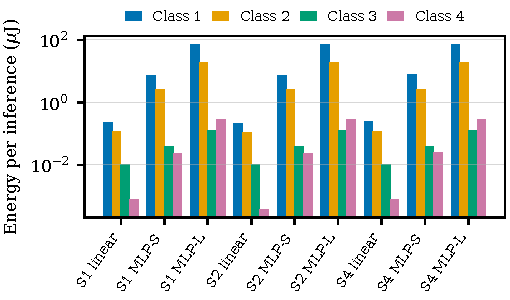
\includegraphics[width=\columnwidth]{fig_energy_inf.pdf}
\caption{Energy of one inference of every model on every platform (log scale). The S3 scorers have the architectures of the S2 models.}
\label{fig:energy_inf}
\end{figure}

\begin{figure}[t]
\centering
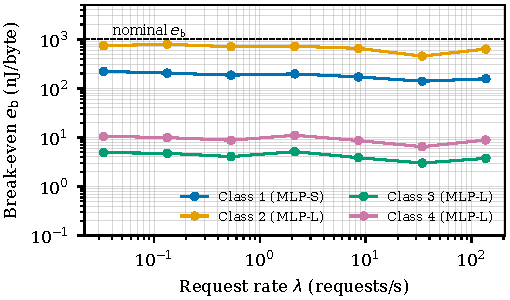
\includegraphics[width=\columnwidth]{fig_breakeven.pdf}
\caption{Backhaul energy per byte above which the selected S2 model reduces the system energy, as a function of the request rate. The dashed line marks the nominal $e_\rmsub{b}$.}
\label{fig:breakeven}
\end{figure}

\subsection{Sensitivity (RQ5)}\label{sec:rq5}

Fig.~\ref{fig:window} shows the windowed hit ratio $H_\ell$ of the baseline and of both pipelines on Class~3 over the test part, which spans two popularity reshuffles. The hit-ratio-oriented pipeline is above the baseline in all 14 full windows, by 3.7 points on average, and the energy-neutral pipeline in 13, by 1.9 points. After the second reshuffle, the gap of $\bpi^\star_p$ closes for about two hours and that of $\bpi^H_p$ narrows to 1.3 points. Both recover without retraining, because the features of S2 and S3 describe the recent requests of each item and the recent transitions between items rather than their identities. Table~\ref{tab:cache} shows how the two pipelines behave as the cache grows from 0.5\% to 5\% of the unique test bytes; the models and pipelines are those selected at the nominal size. On Class~3, both pipelines gain at every size: $\bpi^\star_p$ by 2.5 to 2.9 points and $\bpi^H_p$ by 3.6 to 5.0 points. Relative to the baseline, the gain is largest for small caches, 19\% and 30\% at 0.5\%, where every admission decision matters most. Class~2 behaves like Class~3. On Class~1, the gains shrink as the cache grows and vanish for $\bpi^\star_p$ at 5\%, with a wide confidence interval. The cache index of a larger cache takes RAM from the history, which falls from 2,000 requests at 0.5\% to 1,540 at 5\%, about 48~min of demand, while the larger cache keeps items for longer than that; S2 then sees many cached items without a recorded request. On the smallest platform, memory thus limits the cache size at which a learned admission policy helps.

\begin{figure}[t]
\centering
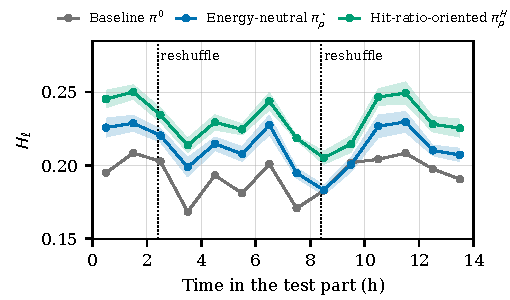
\includegraphics[width=\columnwidth]{fig_window.pdf}
\caption{Hit ratio in consecutive 1-h windows of the test part on Class~3 (mean over five seeds; bands: 95\% confidence interval). Dotted lines mark the popularity reshuffles; the last, partial window is omitted.}
\label{fig:window}
\end{figure}

\begin{table}[t]
\centering
\caption{Gain over $\bpi^0$ against the Cache Size (Synthetic Trace; Percentage Points, Mean over Seeds $\pm$ 95\% Confidence Half-Width)}
\label{tab:cache}
\footnotesize
\setlength{\tabcolsep}{1.8pt}
\begin{tabular}{@{}lccccc@{}}
\toprule
 & & \multicolumn{2}{c}{Class 1} & \multicolumn{2}{c}{Class 3} \\
\cmidrule(lr){3-4}\cmidrule(l){5-6}
$C$ & $H(\bpi^0)$ & $\bpi^\star_p$ & $\bpi^H_p$ & $\bpi^\star_p$ & $\bpi^H_p$ \\
\midrule
0.5\% & 0.129 & $+3.29\pm0.59$ & $+4.20\pm0.23$ & $+2.49\pm0.42$ & $+3.92\pm0.34$ \\
1\% & 0.195 & $+1.85\pm0.65$ & $+2.76\pm0.24$ & $+1.87\pm0.45$ & $+3.64\pm0.36$ \\
2\% & 0.251 & $+1.55\pm0.77$ & $+2.19\pm0.50$ & $+2.92\pm0.57$ & $+5.00\pm0.34$ \\
5\% & 0.359 & $-0.19\pm3.11$ & $+0.82\pm1.69$ & $+2.67\pm0.91$ & $+4.58\pm0.71$ \\
\bottomrule
\multicolumn{6}{@{}l@{}}{\scriptsize $C$: share of the unique test bytes; $H(\bpi^0)$ of Class~3.}
\end{tabular}
\end{table}

\subsection{Results on MovieTweetings}\label{sec:mt}

On MovieTweetings, the baseline $\bpi^0$ reaches $H=0.391$ on the test part, against 0.495 for Belady's rule. The demand is more concentrated than in the synthetic trace: 1\% of the movies receive 43\% of the ratings. We evaluate Classes~1 and~3, which bound the platforms in memory and energy, with three seeds.

The admission stage again pays off. In the energy-neutral pipeline, the selected S2 model, MLP-S on Class~1 and MLP-L on Class~3, raises the hit ratio by $1.07\pm0.18$ points on Class~1 and by $1.25\pm0.32$ points on Class~3, about 3\% in relative terms. It reduces the backhaul load by 1.7\% to 2.0\% and saves 3.6 to 6.4~J. As on the synthetic trace, Class~1 selects the smaller model, because S2 MLP-L loses 11.8~J on it on the validation part; the latency loss is at most 0.01 points, and the memory loss on Class~1 lies between $-0.10$ and $+0.11$ points.

Next-request prediction does not help on this trace. On their own, the S3 models change the validation hit ratio by at most 0.07 points, and behind S2 they lose up to 0.12 points, so no S3 model is selected. The hit-ratio-oriented pipeline therefore coincides with the energy-neutral one up to the choice of S1 and gains 1.14 points on Class~1 and 1.23 points on Class~3. The scorer separates the next movie from the other candidates about as well as on the synthetic trace, with an area under the ROC curve of 0.80, but only 1.6\% of the candidates are the next movie of the user, against 4.4\% on the synthetic trace. At $\theta_3=0.10$, five in six prefetches are wrong. The consecutive ratings of a user are less regular than the successions of the synthetic generator, so the gain of prefetching depends on the trace, whereas the gain of admission and eviction carried over.

\section{Hardware Analysis}\label{sec:hw}

This section explains the results of Section~\ref{sec:results} in terms of the hardware of each platform.

\subsection{Where the Cycles Go}

The models of every stage are small: MLP-L has 4,544 to 4,736 MAC operations, and all of its operators run on the accelerator of Class~3. The DSP instructions of the Cortex-M4 reduce the cycles of the MLPs by a factor of 1.7 to 2.5 with respect to the Cortex-M3, from 56,067 to 24,108 cycles for S2 MLP-L. Most of the cost of an S3 decision lies in the pass over the history. With the full history of 20,000 requests, the pass costs about 265,000 processor cycles on the Cortex-M4 and 342,000 on a single-issue core, against 3,300 accelerator cycles for the eight MLP-S inferences on Class~3. The pass thus takes about 99\% of the cycles of an S3 decision on Classes~2 to~4, and the accelerator cannot shorten it. One S3 decision takes about 1.7~ms on Classes~2 and~3 and 2.0~ms on Class~4, and it costs 26~$\mu$J on Class~3, 131~$\mu$J on Class~4, and 229~$\mu$J on Class~2. On Class~1, the short history makes the pass cheaper, about 33,000 cycles, and the decision takes 1.1~ms. An index of the transitions kept in RAM would replace the pass by a lookup at the cost of memory, which is scarcest on Class~1.

\subsection{When the Accelerator Pays Off}

An accelerator adds a fixed cost to each decision, for configuring it and moving the data, and reduces the cost per MAC operation. Let $n_m$ be the number of MAC operations of model $m$. We describe the processor-only execution by $N^\rmsub{cpu}=N^0_\rmsub{c}+n_m/r_\rmsub{c}$ and the accelerated execution by $N^\rmsub{npu}=N^0_\rmsub{n}+n_m/r_\rmsub{n}$ accelerator cycles plus $N_\rmsub{r}$ residual processor cycles, where $r_\rmsub{c}$ and $r_\rmsub{n}$ are the sustained MAC rates per cycle and $N^0_\rmsub{c}$, $N^0_\rmsub{n}$, and $N_\rmsub{r}$ are fixed costs. By \eqref{eq:latency}, the accelerator reduces the latency if and only if $n_m$ exceeds the crossover
\begin{equation}
n^\times_p=\frac{N^0_\rmsub{n}/\phi^\rmsub{npu}_p+(N_\rmsub{r}-N^0_\rmsub{c})/\phi_p}{1/(r_\rmsub{c}\phi_p)-1/(r_\rmsub{n}\phi^\rmsub{npu}_p)},
\label{eq:crossover}
\end{equation}
provided that the denominator is positive. The energy crossover follows in the same way from \eqref{eq:energy}. 

A least-squares fit of this model to the dense models of Table~\ref{tab:cycles} gives $N^\rmsub{cpu}\approx 626+12.2\,n_m$ cycles on the Cortex-M3, $724+5.13\,n_m$ on the Cortex-M4, and $N^\rmsub{npu}\approx 210+0.238\,n_m$ cycles on the Ethos-U55 with 128 MACs. The accelerator thus sustains about 4.2 MAC operations per cycle, a small fraction of its 128 MAC units, and the configurations with 64 and 256 MACs give almost the same counts (Table~\ref{tab:cycles}), since a fully connected layer at batch size one is limited by the transfer of its weights. With the Cortex-M4 model as the processor and equal clocks, \eqref{eq:crossover} gives $n^\times_p=(N_\rmsub{r}-514)/4.89$. Since Vela does not include the cost of invoking the accelerator, $N_\rmsub{r}$ is the driver overhead per inference: the accelerator is faster for every model unless this overhead exceeds 514 processor cycles, and each further 4.9 cycles of overhead moves the crossover up by one MAC operation.

\subsection{Memory}

Table~\ref{tab:memory} shows how the RAM of each platform is divided among the reserved memory, the models of $\bpi^\star_p$, and the request history. On Class~1, the history is limited to 1,917 requests, which cover about 1~h of demand; on the other classes, it reaches the bound $N^\infty_\rmsub{h}=20{,}000$, which covers 10.4~h. Even the pipeline with MLP-L in all four stages fits on Class~1, with a history of 1,761 requests, because the weights reside in flash and the models need only 1.5~KB of RAM for their activations.

\begin{table}[t]
\centering
\caption{RAM Budget of the Energy-Neutral Pipeline (Seed 1)}
\label{tab:memory}
\small
\setlength{\tabcolsep}{2pt}
\begin{tabular*}{\columnwidth}{@{\extracolsep{\fill}}lccccc@{}}
\toprule
Platform & $M^\rmsub{ram}_p$ & $M^\rmsub{ram}_0$ & Models & History & Span $N_\rmsub{h}/\lambda$ \\
\midrule
Class 1 & 20 & 4.7 & 0.3 & 15.0 (1,917) & 1.0~h \\
Class 2 & 192 & 4.7 & 0.7 & 156.3 (20,000) & 10.4~h \\
Class 3 & 512 & 4.7 & 0.7 & 156.3 (20,000) & 10.4~h \\
Class 4 & 512 & 4.7 & 0.7 & 156.3 (20,000) & 10.4~h \\
\multicolumn{6}{@{}l@{}}{\footnotesize All sizes in KB; history length $N_\rmsub{h}$ in parentheses.}\\
\bottomrule
\end{tabular*}
\end{table}

\subsection{Energy Decomposition}

By \eqref{eq:node_energy}, the energy of the EN consists of inference, model updates, sleep, and retention. In the baseline configuration, the sleep term accounts for more than 98\% of $E_\rmsub{EN}$ on every platform: the 0.28~mA Stop current of the STM32F407 alone costs 48~J over the test part, against 2.4~J for the STM32F103. With the energy-neutral pipeline, inference accounts for 54\% of $E_\rmsub{EN}$ on Class~1 (2.8 of 5.2~J), 12\% on Class~2, 1.3\% on Class~3, and 6.7\% on Class~4. The energy that S2 adds is thus comparable to the sleep energy on Class~1 and negligible on Class~3. The hit-ratio-oriented pipeline adds 0.8~J to the node on Class~3, 3.8~J on Class~4, 20~J on Class~2, and 22~J on Class~1, where it mostly runs S2 MLP-L. The link energy, 815~J for the baseline at the nominal $e_\rmsub{b}$, exceeds the node energy of every platform by at least an order of magnitude. This is why a small hit-ratio gain of S2 can pay for a large increase in node energy, and why the backhaul bytes, not the node, set the price of prefetching at this $e_\rmsub{b}$.

\section{Answers to the Research Questions and Design Guidelines}\label{sec:guidelines}

This section collects the answers that Sections~\ref{sec:results} and~\ref{sec:hw} give to the research questions of Section~\ref{sec:setup}, states the best implementation of each stage, and turns the results into a design procedure.

\subsection{Answers to the Research Questions}

\begin{itemize}
\item RQ1: Only admission and eviction (S2) gains from a tinyML model on its own. It raises the hit ratio by 1.8 to 1.9 points over ARC on the synthetic trace, about 9\%, and by 1.1 to 1.3 points on MovieTweetings, about 3\%, while saving energy on every platform. Popularity prediction (S1) and next-cell prediction (S4) gain nothing. Next-request prediction (S3) lowers the hit ratio by about 2 points on its own, but behind the learned S2 model it raises the hit ratio by about 1.8 points on the synthetic trace; on MovieTweetings, it does not help.
\item RQ2: Little of the gain is lost, and memory matters more than latency. The latency loss of S2 is at most 0.03 points on every platform. Memory limits only Class~1: its history of about 1,900 requests reduces the gain of S3 behind S2 from 1.8 to 0.45 points, and the gain of S2 vanishes when the cache grows to 5\% of the unique bytes.
\item RQ3: Table~\ref{tab:recommend} lists the best model and platform for each stage. The energy-neutral pipeline consists of the selected S2 model, in some seeds with S1, and gains 1.85 to 1.89 points while saving 4 to 10~J. The hit-ratio-oriented pipeline adds S3 behind S2 and gains 3.6 to 3.7 points, about 19\%, on Classes~2 to~4 and 2.8 points on Class~1, at the cost of up to 32\% more backhaul traffic. The stages interact positively, with $I_p$ between $+0.05$ and $+0.12$ points for $\bpi^\star_p$, and S2 is what makes S3 useful, since it filters the prefetches of S3.
\item RQ4: S2 reduces the system energy whenever the backhaul costs more than 4.1~nJ/B on Class~3, 8.8~nJ/B on Class~4, 0.19~$\mu$J/B on Class~1, and 0.70~$\mu$J/B on Class~2. Since every sleep mode retains the whole RAM, no minimum request rate exists. Prefetching has no break-even point, because it adds backhaul bytes: it costs about 0.23~J per additional hit at 1~$\mu$J/B, and on a backhaul of 0.1~$\mu$J/B the platform decides much of the price, 24~J on Class~3 against 42~J on Class~2. Up to 136~requests/s, no S2 decision misses its deadline in $\bpi^\star_p$, and the hit-ratio-oriented pipeline loses 0.23 points to latency only on Class~2.
\item RQ5: In relative terms, the gains are largest for small caches, 19\% for $\bpi^\star_p$ and 30\% for $\bpi^H_p$ at 0.5\% of the unique bytes on Class~3, and they persist across popularity reshuffles without retraining. On Class~1, a larger cache index leaves less RAM for the history, and the gain of S2 vanishes at 5\%.
\end{itemize}

Of the hypotheses, H1 is supported, since the energy of one inference of the same model differs by a factor of 189 to 577 across the platforms. H2 holds in its threshold but not in its mechanism: $\Delta H_2$ varies by 20\% across the platforms because of memory, not because of the deadline of S2. H3 is not supported, since the interaction is positive.

\subsection{Recommended Implementation of Each Stage}

\begin{table}[t]
\centering
\caption{Recommended Implementation of Each Stage}
\label{tab:recommend}
\footnotesize
\setlength{\tabcolsep}{2pt}
\begin{tabular*}{\columnwidth}{@{\extracolsep{\fill}}llll@{}}
\toprule
Stage & Model & Platform & Gain and condition \\
\midrule
S1 & Baseline & Any & No model gains \\
S2 & MLP-L$^\ast$ & Class~3 & $+1.9$ / $+1.3$ pts; $e_\rmsub{b}>4.1$~nJ/B \\
S3 & MLP-S or MLP-L & Class~3 & $+1.8$ pts behind S2; regular successions \\
S4 & Baseline & Any & No model gains \\
\bottomrule
\multicolumn{4}{@{}l@{}}{\scriptsize $^\ast$MLP-S on Class~1. Gains: synthetic / MovieTweetings trace.}
\end{tabular*}
\end{table}

Table~\ref{tab:recommend} summarizes the answer to RQ3 for a designer. For a single node, Class~3 is the best platform for both pipelines: it matches the hit ratio of Classes~2 and~4 at the lowest node energy, 0.05~J for S2 and 0.8~J for the hit-ratio-oriented pipeline over the 14.4-h test part, and it gives S3 the cheapest decisions, 26~$\mu$J each. Class~4 is a close second. Class~1 can host S2 with MLP-S on links that cost at least 0.19~$\mu$J per byte and with caches of up to about 2\% of the unique bytes. Class~2 matches the hit ratio of the accelerated classes, but its slow wake-up from sleep makes it the most expensive choice for every stage.

\subsection{Design Procedure}

The model of Sections~\ref{sec:system} and~\ref{sec:problem} gives a procedure for deciding whether to implement a caching stage with tinyML on a given platform before running a full simulation. The procedure uses only quantities that a designer can obtain from the trace and from compiling the model.
\begin{enumerate}
\item Estimate the request rate $\lambda$ of the node, the trigger rate $\lambda_j$ of each stage, and the mean fetch delay, which bounds the deadline $\delta_2$ of S2.
\item Compile each candidate model for the platform, check the feasibility conditions of Definition~\ref{def:feasible}, and compute the history length $N_\rmsub{h}$ that the remaining RAM allows.
\item Compute $\tau_{m,p}$ from \eqref{eq:latency} and the load $\rho_p(\bpi)$ from \eqref{eq:utilization}. Discard any configuration with $\rho_p(\bpi)\ge1$, and discard any S2 model whose decision latency $(1+n_\rmsub{e})\tau_{m,p}$ exceeds the typical fetch delay, since its decisions would be dropped.
\item Estimate $\Delta h$ from a zero-latency simulation, compute the margin $\Gamma_j$ from \eqref{eq:margin}, and discard the model if $\Gamma_j\le0$ or if $\lambda\le\lambda^\star_j$.
\item Simulate only the remaining configurations, and among them solve \eqref{eq:combined}.
\end{enumerate}
Steps 1 to 4 require no simulation of the platform, and they remove the configurations that cannot pay off. In applying them, the designer should count the work outside the model, such as the pass of S3 over the history, and the wake-up of the processor, which made every decision expensive on Class~2; a small accelerator of 64 MAC units is enough for these models.

\section{Threats to Validity}\label{sec:threats}

\subsection{Internal Validity}

The decision latencies come from sources of different accuracy: modelled instruction timings that neglect bus contention on Classes~1 and~2, compiler estimates without driver overhead on Class~3 \cite{arm_vela}, and the throughput of a convolutional network on Class~4, which may differ from that of small fully connected layers. These errors affect the results only through the staleness and the deadlines of Section~\ref{sec:timing}. With S2 alone, the highest processor load in the study was 0.27 and no decision missed its deadline; the hit-ratio-oriented pipeline reached 0.63 on Class~2 at 136~requests/s, where 192 decisions missed theirs. An error of a factor of two in the latencies would therefore not change the results at the nominal rate, but it could change the latency loss at the highest rates; it would change the node energy proportionally.

The simulator computes the decisions on the host. Their agreement with the int8 models was checked in the reference interpreter; the comparison with the compiled firmware remains to be done. The models were trained with the longest history $N^\infty_\rmsub{h}$ and deployed with the history that each platform allows, so on Class~1 their inputs differ from their training inputs.

\subsection{Construct Validity}

The energy of the EN is modelled, not measured. The model \eqref{eq:energy} is linear in the cycle counts and uses currents at one operating point, so it does not capture the dependence of the current on the executed instructions or on the temperature. The accelerator energy of Class~3 is derived from vendor ratios, and the energy of Class~4 is an average over a whole network at one operating point. The link parameters and energies are assumptions; we therefore report the break-even backhaul energy rather than a single verdict.

The delay model assumes store-and-forward transfers and uncongested links (Assumption~\ref{as:links}). Store-and-forward overestimates the delay of a miss compared with a node that forwards bytes as they arrive, so the reported reductions in delay are upper bounds on those of such a node. Belady's rule is reported as a reference and is not an upper bound for items of different sizes. The hit ratio and the byte hit ratio measure the caching performance but not the quality of experience of the users.

\subsection{External Validity}

The results come from two traces. The synthetic trace was generated with chosen parameters, and S3 and S4 can only exploit the regularities that the generator puts into the requests; the precision of S3, for example, is bounded by the successor probabilities of the generator. MovieTweetings records real demand, but a rating is only a proxy for a request, the dataset has no item sizes or user locations, and time scaling compresses its temporal structure. Neither trace was recorded at an IoT edge node. A CDN trace such as the Wikipedia trace released with LRB \cite{song2020} would test the admission stage on objects of different sizes.

The study considers one EN, one representative device per platform class, and one operating point per device. Cooperation among several nodes, voltage and frequency scaling, and other devices of the same class may change the results. The candidate models are linear models and MLPs; recurrent and convolutional models, as well as gradient-boosted trees, are not covered.

\subsection{Conclusion Validity}

Each configuration is evaluated with five training seeds on the synthetic trace and three on MovieTweetings, which still gives wide confidence intervals for small gains. We therefore compare configurations through paired differences and report confidence intervals instead of single values. Model, threshold, and pipeline selection use only the validation part, and the test part is used once, which prevents the selection from fitting the test data. The hypotheses and their thresholds were fixed before the experiments. Since many stage and platform pairs are compared, some differences will appear significant by chance, and we report all comparisons rather than only the significant ones.

\section{Conclusion}\label{sec:conclusion}

This paper studied how much of the gain of a tinyML caching model survives on the hardware of a low-power edge cache node. We modelled the caching decisions as a pipeline of four stages, described each platform by a profile of its speed, memory, and energy, and represented the time of every decision through an explicit queue. On this model we built a benchmark that selects the best model and platform for each stage, builds an energy-neutral and a hit-ratio-oriented pipeline, and separates the loss caused by latency from the loss caused by memory, and we derived the condition under which a tinyML stage reduces the energy of the system. All hardware figures come from datasheets, published measurements, compiler estimates, and instruction-level models, so the results can be reproduced without the boards.

Admission and eviction was the only stage that paid off on its own. Its learned model raised the hit ratio by about 1.8 points over ARC on a synthetic trace and by 1.1 to 1.3 points on a trace of real movie ratings, while saving energy. Next-request prefetching helped only behind this learned admission stage and only where the demand had regular successions: on the synthetic trace, the two stages together gained up to 3.7 points, about 19\%, at the cost of up to 32\% more backhaul traffic, whereas on the movie ratings prefetching did not help. The platform hardly changed the hit-ratio gain, but it set its energy cost. The energy of one inference differed by up to 577 times across the platforms, and admission and eviction saved energy above 4~nJ per backhaul byte on the platform with a neural accelerator, against 0.7~$\mu$J on the Cortex-M4. A microcontroller with a small neural accelerator is therefore the natural host for learned caching decisions, and the smallest platform can host only the smaller admission model on costly links.

The next steps are results on CDN traces with items of different sizes and the validation of the cycle and energy models on hardware. Delivering a semantically similar cached item in place of a missing one, cooperation among several nodes, congested links, and on-device training are further extensions.

\section*{Code and Data Availability}

The simulator, the platform profiles, the trained models, the cycle model, the synthetic trace, the MovieTweetings window used here, and the scripts that produce every table and figure are available at \url{https://github.com/sshawky78AUA/tinyML-Edge-Caching}. The MovieTweetings dataset is available from its authors \cite{dooms2013}.

\begin{thebibliography}{99}
\bibitem{sanchez2020}
R.~Sanchez-Iborra and A.~F. Skarmeta, ``TinyML-enabled frugal smart objects: Challenges and opportunities,'' \emph{IEEE Circuits Syst. Mag.}, vol.~20, no.~3, pp.~4--18, 2020.

\bibitem{david2021}
R.~David \emph{et~al.}, ``TensorFlow Lite Micro: Embedded machine learning for TinyML systems,'' in \emph{Proc. Mach. Learn. Syst. (MLSys)}, vol.~3, 2021.

\bibitem{banbury2021}
C.~Banbury \emph{et~al.}, ``MLPerf Tiny benchmark,'' in \emph{Proc. Neural Inf. Process. Syst. Track Datasets Benchmarks}, 2021.

\bibitem{jacob2018}
B.~Jacob \emph{et~al.}, ``Quantization and training of neural networks for efficient integer-arithmetic-only inference,'' in \emph{Proc. IEEE/CVF Conf. Comput. Vis. Pattern Recognit. (CVPR)}, 2018, pp.~2704--2713.

\bibitem{lai2018}
L.~Lai, N.~Suda, and V.~Chandra, ``CMSIS-NN: Efficient neural network kernels for Arm Cortex-M CPUs,'' arXiv:1801.06601, 2018.

\bibitem{lin2020}
J.~Lin, W.-M. Chen, Y.~Lin, J.~Cohn, C.~Gan, and S.~Han, ``MCUNet: Tiny deep learning on IoT devices,'' in \emph{Proc. Adv. Neural Inf. Process. Syst. (NeurIPS)}, vol.~33, 2020.

\bibitem{kusupati2018}
A.~Kusupati, M.~Singh, K.~Bhatia, A.~Kumar, P.~Jain, and M.~Varma, ``FastGRNN: A fast, accurate, stable and tiny kilobyte sized gated recurrent neural network,'' in \emph{Proc. Adv. Neural Inf. Process. Syst. (NeurIPS)}, 2018, pp.~9017--9028.

\bibitem{flamand2018}
E.~Flamand, D.~Rossi, F.~Conti, I.~Loi, A.~Pullini, F.~Rotenberg, and L.~Benini, ``GAP-8: A RISC-V SoC for AI at the edge of the IoT,'' in \emph{Proc. IEEE 29th Int. Conf. Appl.-Specific Syst., Archit. Processors (ASAP)}, Milan, Italy, 2018, pp.~1--4.

\bibitem{golrezaei2013}
N.~Golrezaei, A.~F. Molisch, A.~G. Dimakis, and G.~Caire, ``Femtocaching and device-to-device collaboration: A new architecture for wireless video distribution,'' \emph{IEEE Commun. Mag.}, vol.~51, no.~4, pp.~142--149, Apr. 2013.

\bibitem{bastug2014}
E.~Ba\c{s}tu\u{g}, M.~Bennis, and M.~Debbah, ``Living on the edge: The role of proactive caching in 5G wireless networks,'' \emph{IEEE Commun. Mag.}, vol.~52, no.~8, pp.~82--89, Aug. 2014.

\bibitem{shi2016}
W.~Shi, J.~Cao, Q.~Zhang, Y.~Li, and L.~Xu, ``Edge computing: Vision and challenges,'' \emph{IEEE Internet Things J.}, vol.~3, no.~5, pp.~637--646, Oct. 2016.

\bibitem{hosny2016allerton}
S.~Hosny, A.~Eryilmaz, A.~A. Abouzeid, and H.~El~Gamal, ``Mobility-aware centralized D2D caching networks,'' in \emph{Proc. 54th Annu. Allerton Conf. Commun., Control, Comput.}, Monticello, IL, USA, 2016, pp.~725--732.

\bibitem{hosny2016globecom}
S.~Hosny, A.~Eryilmaz, and H.~El~Gamal, ``Impact of user mobility on D2D caching networks,'' in \emph{Proc. IEEE Global Commun. Conf. (GLOBECOM)}, Washington, DC, USA, 2016, pp.~1--6.

\bibitem{thar2018}
K.~Thar, N.~H. Tran, T.~Z. Oo, and C.~S. Hong, ``DeepMEC: Mobile edge caching using deep learning,'' \emph{IEEE Access}, vol.~6, pp.~78260--78275, 2018.

\bibitem{kianfar2025}
G.~Kianfar, Z.~Hajiakhondi-Meybodi, and A.~Mohammadi, ``CacheMamba: Popularity prediction for mobile edge caching networks via selective state spaces,'' arXiv:2502.15746, 2025.

\bibitem{song2020}
Z.~Song, D.~S. Berger, K.~Li, and W.~Lloyd, ``Learning relaxed Belady for content distribution network caching,'' in \emph{Proc. 17th USENIX Symp. Netw. Syst. Design Implement. (NSDI)}, Santa Clara, CA, USA, 2020, pp.~529--544.

\bibitem{chang2018}
Z.~Chang, L.~Lei, Z.~Zhou, S.~Mao, and T.~Ristaniemi, ``Learn to cache: Machine learning for network edge caching in the big data era,'' \emph{IEEE Wireless Commun.}, vol.~25, no.~3, pp.~28--35, Jun. 2018.

\bibitem{shuja2021}
J.~Shuja, K.~Bilal, W.~Alasmary, H.~Sinky, and E.~Alanazi, ``Applying machine learning techniques for caching in next-generation edge networks: A comprehensive survey,'' \emph{J. Netw. Comput. Appl.}, vol.~181, Art. no.~103005, 2021.

\bibitem{dooms2013}
S.~Dooms, T.~De~Pessemier, and L.~Martens, ``MovieTweetings: A movie rating dataset collected from Twitter,'' in \emph{Proc. Workshop Crowdsourcing Human Comput. Recommender Syst. (CrowdRec) at ACM RecSys}, Hong Kong, 2013.

\bibitem{maddahali2014}
M.~A. Maddah-Ali and U.~Niesen, ``Fundamental limits of caching,'' \emph{IEEE Trans. Inf. Theory}, vol.~60, no.~5, pp.~2856--2867, May 2014.

\bibitem{belady1966}
L.~A. Belady, ``A study of replacement algorithms for a virtual-storage computer,'' \emph{IBM Syst. J.}, vol.~5, no.~2, pp.~78--101, 1966.

\bibitem{megiddo2003}
N.~Megiddo and D.~S. Modha, ``ARC: A self-tuning, low overhead replacement cache,'' in \emph{Proc. 2nd USENIX Conf. File Storage Technol. (FAST)}, San Francisco, CA, USA, 2003.

\bibitem{yang2020}
J.~Yang, Y.~Yue, and K.~V. Rashmi, ``A large scale analysis of hundreds of in-memory cache clusters at Twitter,'' in \emph{Proc. 14th USENIX Symp. Oper. Syst. Design Implement. (OSDI)}, 2020, pp.~191--208.

\bibitem{bruschi2021}
N.~Bruschi, G.~Haugou, G.~Tagliavini, F.~Conti, L.~Benini, and D.~Rossi, ``GVSoC: A highly configurable, fast and accurate full-platform simulator for RISC-V based IoT processors,'' in \emph{Proc. IEEE 39th Int. Conf. Comput. Design (ICCD)}, 2021, pp.~409--416.

\bibitem{karras2024}
A.~Karras, A.~Giannaros, C.~Karras, L.~Theodorakopoulos, C.~S. Mammassis, G.~A. Krimpas, and S.~Sioutas, ``TinyML algorithms for big data management in large-scale IoT systems,'' \emph{Future Internet}, vol.~16, no.~2, Art. no.~42, 2024.

\bibitem{st_f103}
STMicroelectronics, ``STM32F103x8, STM32F103xB: Medium-density performance line Arm-based 32-bit MCU with 64 or 128~KB flash, USB, CAN, 7 timers, 2 ADCs, 9 communication interfaces,'' Datasheet DS5319. [Online]. Available: \url{https://www.st.com/en/microcontrollers-microprocessors/stm32f103rb.html}

\bibitem{arm_m55blog}
Arm Ltd., ``Arm Cortex-M55 and Ethos-U55 processors: Extending the performance of Arm's ML portfolio for endpoint devices,'' Arm Community Blog, Feb. 2020. [Online]. Available: \url{https://developer.arm.com/community/arm-community-blogs/b/architectures-and-processors-blog/posts/cortex-m55-and-ethos-u55-processors-extending-the-performance-of-arm-ml-portfolio-for-endpoint-devices}

\bibitem{st_f407}
STMicroelectronics, ``STM32F405xx, STM32F407xx: Arm Cortex-M4 32b MCU+FPU, 210 DMIPS, up to 1~MB flash/192+4~KB RAM, USB OTG HS/FS, Ethernet, 17 TIMs, 3 ADCs, 15 comm. interfaces \& camera,'' Datasheet DS8626, Rev.~12, Mar. 2026.

\bibitem{alif_e3}
Alif Semiconductor, ``Ensemble E3 series embedded microcontrollers,'' Datasheet, v2.9. [Online]. Available: \url{https://www.mouser.com/datasheet/2/1549/Alif_E3_Datasheet_v2_9-3454193.pdf}

\bibitem{gap8_web}
GreenWaves Technologies, ``GAP8 and GAP9 processors.'' [Online]. Available: \url{https://greenwaves-technologies.com/?p=4526}

\bibitem{garofalo2020}
A.~Garofalo, M.~Rusci, F.~Conti, D.~Rossi, and L.~Benini, ``PULP-NN: Accelerating quantized neural networks on parallel ultra-low-power RISC-V processors,'' \emph{Philos. Trans. R. Soc. A}, vol.~378, no.~2164, Art. no.~20190155, 2020.

\bibitem{arm_vela}
Arm Ltd., ``Vela: Neural network model compiler for Arm Ethos-U NPUs.'' [Online]. Available: \url{https://pypi.org/project/ethos-u-vela/}

\bibitem{alif_slides}
Alif Semiconductor, ``Supplying next generation microcontrollers: How Alif innovated solutions turn edge AI into reality,'' presentation, Tech Taipei Embedded, Jul. 2024. [Online]. Available: \url{https://site.eettaiwan.com/events/tech_taipei_embedded24/images/download/06-How-ALIF-Innovated-Solutions-Turn-Edge-AI-Into%20Reality-July-2024.pdf}

\bibitem{bellard2005}
F.~Bellard, ``QEMU, a fast and portable dynamic translator,'' in \emph{Proc. USENIX Annu. Tech. Conf., FREENIX Track}, Anaheim, CA, USA, 2005, pp.~41--46.

\bibitem{arm_m3trm}
Arm Ltd., \emph{Cortex-M3 Technical Reference Manual}, ARM DDI 0337G, 2008.

\bibitem{arm_m4trm}
Arm Ltd., \emph{Cortex-M4 Technical Reference Manual}, ARM DDI 0439B, 2010.

\bibitem{arm_fastmodels}
Arm Ltd., ``Fast Models reference guide: Model capabilities,'' Document 100964. [Online]. Available: \url{https://developer.arm.com/documentation/100964/1116/Introduction-to-the-Fast-Models-Reference-Manual/Model-capabilities}

\bibitem{alif_web}
Alif Semiconductor, ``Ensemble E3 series.'' [Online]. Available: \url{https://alifsemi.com/ensemble-e3-series/}

\bibitem{che2002}
H.~Che, Y.~Tung, and Z.~Wang, ``Hierarchical web caching systems: Modeling, design and experimental results,'' \emph{IEEE J. Sel. Areas Commun.}, vol.~20, no.~7, pp.~1305--1314, Sep. 2002.

\bibitem{kleinrock1975}
L.~Kleinrock, \emph{Queueing Systems, Volume 1: Theory}. New York, NY, USA: Wiley, 1975.

\end{thebibliography}

\end{document}
